\subsection{Discrete valuations}

DEFINITION 3. Let K be a (not necessarily commutative) field, v a valuation on K and \(\Gamma\) the order group of v. v is called discrete if there exists a (necessarily unique) isomorphism of the ordered group \(\Gamma\) onto Z. Let \(\gamma\) be the element of \(\Gamma\) corresponding to 1 under this isomorphism; every element u of K such that \(v(u) = \gamma\) is called a uniformizer of v. A discrete valuation is called normed if its order group is Z.

For example the valuation \(v_{p}\) defined by an extremal element p of a principal ideal *or factorial* domain is a normed discrete valuation which admits p as a uniformizer. In particular, if k is a field, \(k[[T]]\) is the ring of a discrete valuation on \(k((T))\) which admits T as a uniformizer. * Let S be a connected complex analytic variety of dimension 1, K the field of meromorphic functions on S and \(z_{0}\) a point of S; the set of \(f \in K\) which are holomorphic at \(z_{0}\) is the ring of a discrete valuation v; for a function \(f \in K\) to be uniformizing for v, it is necessary and sufficient that it be holomorphic and zero at \(z_{0}\) and that there exist a neighbourhood V of \(z_{0}\) in S such that the restriction of f to V be a homomorphism of V onto a neighbourhood of the origin in C. It is this example and other analogues which are the origin of the word ``uniformizer''.*

PROPOSITION 8. Let K be a (not necessarily commutative) field, v a discrete valuation on K, A the ring of v and u a uniformizer for v. The non-zero ideals of A are two-sided and of the form Au \(^{n}\) (n ≥ 0).

It may be assumed that \(v\) is normed, so that \(v(u) = 1\) . For all \(x \in \mathbf{K}^*\) , there is an integer \(n \in \mathbf{Z}\) such that \((v(x) = n = v(u^n))\) and hence we may write

\[
x = z u ^ {n} = u ^ {n} z ^ {\prime},
\]

where \(z, z'\) are two invertible elements of the ring A; whence the proposition.

PROPOSITION 9. Let A be a local integral domain distinct from its field of fractions. The following conditions are equivalent:

\begin{enumerate}
\def\labelenumi{(\alph{enumi})}
\item
  A is the ring of a discrete valuation.
\item
  A is a principal ideal domain.
\item
  The ideal \(\mathfrak{m}(\mathbf{A})\) is principal and \(\bigcap_{n=1}^{\infty} \mathfrak{m}(\mathbf{A})^n = (0)\) .
\item
  A is a Noetherian ring and \(\mathfrak{m}(\mathbf{A})\) is principal.
\item
  A is a Noetherian valuation ring.
\end{enumerate}

Proposition 8 shows that (a) implies (b), (d) and (e). If A is a principal ideal domain, then \(\mathfrak{m}(\mathbf{A}) = \mathbf{A}\mathbf{u}\) and every non-zero ideal of A is of the form \(\mathbf{A}\mathbf{u}^n\) since A is local (Algebra, Chapter VII, §1, no. 3, Theorem 2); therefore \(\bigcap_{n=1}^{\infty} \mathfrak{m}(A)^n = 0\) ; this shows that (b) implies (c). On the other hand (d) implies (c) (Chapter III, §3, no. 2, Corollary to Proposition 5); by Proposition 2 of §1, no. 4, (c) implies (a). Thus conditions (a), (b), (c), (d) are equivalent and imply (e). Finally suppose (e) holds and let us show that (b) holds; it will be sufficient to prove the following lemma:

LEMMA 1. Let A be a valuation ring. Every finitely generated torsion-free A-module is free. Every finitely generated ideal of A is principal. Every torsion-free A-module is flat.

Let E be a finitely generated torsion-free A-module and let \(x_{1}, \ldots, x_{n}\) be generators of E which are minimal in number; we show that they are linearly independent. If \(\sum_{i=1}^{n} a_i x_i = 0\) ( \(a_i \in A\) ) is a non-trivial relation between the \(x_i\) , one of the \(a_i\) , say \(a_1\) , divides all the others since the set of principal ideals of \(A\) is totally ordered by inclusion (§ 1, no. 2, Theorem 1); then \(a_1 \neq 0\) since the relation is non-trivial. As \(E\) is torsion-free, we can divide by \(a_1\) , which amounts to assuming that \(a_1 = 1\) . But then \(x_1\) is a linear combination of \(x_2, \ldots, x_n\) , contrary to the minimal character of \(n\) . Hence \(E\) is free.

In particular every finitely generated ideal a of A is principal, all the elements of a system of generators of a being multiples of one of them. Proposition 3 of Chapter I, § 2, no. 4 then shows that every torsion-free A-module is flat.

\section{THE HEIGHT OF A VALUATION}

\subsection{Inclusion of valuation rings of the same field}

PROPOSITION 1. Let K be a field and A a valuation ring of K. Then:

\begin{enumerate}
\def\labelenumi{(\alph{enumi})}
\item
  Every ring \(\mathbf{B}\) such that \(\mathbf{A} \subset \mathbf{B} \subset \mathbf{K}\) is a valuation ring of \(\mathbf{K}\) ;
\item
  The maximal ideal \(\mathfrak{m}(\mathbf{B})\) of such a ring is contained in \(\mathbf{A}\) and it is a prime ideal of \(\mathbf{A}\) ;
\item
  The mapping \(\mathfrak{p} \mapsto \mathbf{A}_{\mathfrak{p}}\) is a decreasing bijection of the set of prime ideals of \(\mathbf{A}\) onto the set of rings \(\mathbf{B}\) such that \(\mathbf{A} \subset \mathbf{B} \subset \mathbf{K}\) ; its inverse bijection is the mapping \(\mathbf{B} \mapsto \mathfrak{m}(\mathbf{B})\) .
\end{enumerate}

If B is a ring such that \(A \subset B \subset K\) and \(x \in K - B\) , then \(x \in K - A\) , whence \(x^{-1} \in \mathfrak{m}(A) \subset B\) , which proves both that B is a valuation ring of K and that \(\mathfrak{m}(B) \subset \mathfrak{m}(A)\) ; as \(\mathfrak{m}(B) = \mathfrak{m}(B) \cap A\) is a prime ideal of A, we have shown (a)

and (b). Moreover, \(\mathbf{A}_{\mathfrak{m}(\mathbf{B})} \subset \mathbf{B}\) ; conversely, if \(x \in \mathbf{B} - \mathbf{A}\) , then \(x^{-1} \in \mathbf{A}\) and \(x^{-1} \notin \mathfrak{m}(\mathbf{B})\) and hence \(x \in \mathbf{A}_{\mathfrak{m}(\mathbf{B})}\) ; thus \(\mathbf{A}_{\mathfrak{m}(\mathbf{B})} = \mathbf{B}\) . Finally let \(\mathfrak{p}\) be a prime ideal of \(\mathbf{A}\) ; we write \(\mathbf{B} = \mathbf{A}_{\mathfrak{p}}\) ; then \(\mathfrak{m}(\mathbf{B}) \cap \mathbf{A} = \mathfrak{p}\) . (Chapter II, §2, no. 5, Proposition 11) and \(\mathfrak{m}(\mathbf{B}) \subset \mathbf{A}\) by (b); hence \(\mathfrak{m}(\mathbf{B}) = \mathfrak{p}\) , which shows that the mappings \(\mathfrak{p} \mapsto \mathbf{A}_{\mathfrak{p}}\) and \(\mathbf{B} \mapsto \mathfrak{m}(\mathbf{B})\) of the statement are inverse bijections.

COROLLARY. The set of subrings of K containing A is totally ordered by inclusion.

The set of prime ideals of A is totally ordered by inclusion (§ 1, no. 2, Theorem 1 (e)) and the mapping \(\mathfrak{p} \mapsto \mathrm{A}_{\mathfrak{p}}\) reverses the inclusion relations.

PROPOSITION 2. Let K be a field, B a valuation ring of K and \(h_B\) the place of K associated with B (with values in \(\kappa(B)\) ). Then the mapping \(A \mapsto h_B(A)\) defines a bijection of the set \(\mathfrak{A}\) of valuation rings of K contained in B onto the set \(\mathfrak{A}'\) of valuation rings of \(\kappa(B)\) .

If \(\mathbf{A} \in \mathfrak{A}\) , then \(h_{\mathrm{B}}(\mathbf{A}) \in \mathfrak{A}'\) : for if \(x' = h_{\mathrm{B}}(x)\) (where \(x \in \mathbf{B}\) ) is an element of \(\kappa(\mathbf{B}) - h_{\mathrm{B}}(\mathbf{A})\) , then \(x \notin \mathbf{A}\) , hence \(x^{-1} \in \mathbf{A}\) and \(h_{\mathrm{B}}(x)^{-1} \in h_{\mathrm{B}}(\mathbf{A})\) . On the other hand, for \(\mathbf{A} \in \mathfrak{A}\) , \(\mathbf{A} \supset \mathfrak{m}(\mathbf{B})\) (Proposition 1 (b)) and hence the mapping, \(\mathbf{A} \mapsto h_{\mathrm{B}}(\mathbf{A})\) is injective. Finally, let \(\mathbf{A}' \in \mathfrak{A}'\) and \(\mathbf{A} = \bar{h}_{\mathrm{B}}^{-1}(\mathbf{A}') \subset \mathbf{B}\) ; we shall show, which will complete the proof, that \(\mathbf{A} \in \mathfrak{A}\) ; if \(x \in \mathbf{K} - \mathbf{A}\) , then either \(x \notin \mathbf{B}\) , or \(x \in \mathbf{B}\) ; if \(x \notin \mathbf{B}\) , then \(x^{-1} \in \mathfrak{m}(\mathbf{B}) \subset \mathbf{A}\) ; if \(x \in \mathbf{B}\) , then \(h_{\mathrm{B}}(x) \in \kappa(\mathbf{B})\) and \(h_{\mathrm{B}}(x) \notin \mathbf{A}'\) , hence \(h_{\mathrm{B}}(x^{-1}) \in \mathbf{A}'\) and we conclude again that \(x^{-1} \in \mathbf{A}\) ; hence \(\mathbf{A} \in \mathfrak{A}\) .

COROLLARY. Let A and B be two valuation rings of K, where \(A \subset B\) ; let \(A' = h_{B}(A)\) , which is a valuation ring of \(\kappa(B)\) . The residue field \(\kappa(A')\) of \(A'\) is canonically isomorphic to the residue field \(\kappa(A)\) of A and the place \(h_{A}\) associated with A is the composition \(h_{A'} \circ h_{B}\) of the places associated with \(A'\) and B.

Since the local ring A' is a quotient of the local ring A, their residue fields are canonically isomorphic and the equation \(h_{\mathrm{A}}(x) = h_{\mathrm{A}'}(h_{\mathrm{B}}(x))\) holds for \(x \in A\) . On the other hand, if \(x \in B - A\) , then \(h_{\mathrm{B}}(x) \notin A'\) and the two sides of the equation are equal to \(\infty\) ; the same is true if \(x \in K - B\) .

Remark. Conversely, let \(f\) be a place of \(\mathbf{K}\) with values in \(\mathbf{K}'\) and \(f'\) a place of \(\mathbf{K}'\) with values in \(\mathbf{K}''\) . Then \(f' \circ f\) is a place of \(\mathbf{K}\) whose ring is contained in the ring of the place \(f\) .

\subsection{Isolated subgroups of an ordered group}

To study the situation in no. 1 from the point of view of valuations we shall need Definition 1 and Proposition 3 below.

DEFINITION 1. A subgroup H of an ordered group G is called isolated if the relations \(0 \leqslant y \leqslant x\) and \(x \in \mathbf{H}\) imply \(y \in \mathbf{H}\) .

Example (1) Let A and B be two ordered groups; let \(A \times B\) be given the lexicographic order (i.e.~`` \((a, b) \leqslant (a', b')\) '' is equivalent to `` \((a < a')\) or \((a = a' \text{ and } b \leqslant b')\) ''). The second factor B of \(A \times B\) is then, as is seen immediately, an isolated subgroup of \(A \times B\) .

PROPOSITION 3. Let G be an ordered group and P the set of its positive elements.

\begin{enumerate}
\def\labelenumi{(\alph{enumi})}
\item
  The kernel of an increasing homomorphism of G to an ordered group is an isolated subgroup of G.
\item
  Conversely, let H be an isolated subgroup of G and g the canonical homomorphism of G onto G/H. Then \(g(P)\) is the set of positive elements of an ordered group structure on G/H. Moreover, if G is totally ordered, so is G/H.
\item
  Let \(f\) be an increasing homomorphism from \(G\) to an ordered group; let \(H\) denote the kernel of \(f\) . If \(0 \leqslant y \leqslant x\) and \(x \in H\) , then \(0 \leqslant f(y) \leqslant f(x) = 0\) , whence \(f(y) = 0\) , that is \(y \in H\) . Hence \(H\) is isolated.
\item
  Let \(\mathbf{H}\) be an isolated subgroup of \(\mathbf{G}\) and \(g\colon \mathbf{G}\to \mathbf{G} / \mathbf{H}\) . Let \(\mathbf{P}' = g(\mathbf{P})\) . Clearly \(\mathbf{P}' + \mathbf{P}'\subset \mathbf{P}'\) . Also
\end{enumerate}

\[
\mathrm{P} ^ {\prime} \cap (- \mathrm{P} ^ {\prime}) = \{0 \},
\]

for, if \(x\) and \(y\) are elements of \(\mathbf{P}\) such that \(g(x) = -g(y)\) , then \(x + y \in \mathbf{H}\) , whence \(x \in \mathbf{H}\) and \(y \in \mathbf{H}\) since \(\mathbf{H}\) is isolated; hence \(g(x) = g(y) = 0\) . Thus \(\mathbf{P}'\) is the set of positive elements of an ordered group structure on \(\mathbf{G} / \mathbf{H}\) (Algebra, Chapter VI, §1, no. 3, Proposition 3). Finally, if \(\mathbf{G}\) is totally ordered, then \(\mathbf{P} \cap (-\mathbf{P}) = \mathbf{G}\) , whence \(\mathbf{P}' \cup (-\mathbf{P}') = \mathbf{G} / \mathbf{H}\) and therefore \(\mathbf{G} / \mathbf{H}\) is totally ordered (loc. cit.).

Example (2) If we reconsider the example where G is a lexicographic product \(A \times B\) and H = B, the ordered group G/H is canonically identified with A.

\subsection{Comparison of valuations}

Let K be a field and A a valuation ring of K. For every subring B of K containing A, \(U(A) \subset U(B)\) . Then there is a canonical homomorphism \(\lambda\) of \(\Gamma_{A} = K^{*}/U(A)\) onto \(\Gamma_{B} = K^{*}/U(B)\) , whose kernel is \(U(B)/U(A)\) . Then, letting \(v_{A}\) and \(v_{B}\) denote the canonical valuations on K defined by A and B ( \(\S 3\) , no. 2),

\[
v _ {\mathrm{B}} = \lambda \circ v _ {\mathrm{A}}.\tag{1}
\]

As \(A \subset B\) , \(\lambda\) maps the positive elements of \(\Gamma_{A}\) to positive elements of \(\Gamma_{B}\) and hence is increasing. Therefore (Proposition 3) the kernel \(H_{B}\) of \(\lambda\) is an isolated subgroup of \(\Gamma_{A}\) and \(\lambda\) factors into \(\Gamma_{A} \to \Gamma_{A}/H_{B} \xrightarrow{\mu} \Gamma_{B}\) , where \(\mu\) is an increasing bijective homomorphism and hence an isomorphism of totally ordered groups; hence \(\Gamma_{B}\) is identified with the quotient totally ordered group \(\Gamma_{A}/H_{B}\) .

PROPOSITION 4. The mapping \(\mathbf{B} \mapsto \mathbf{H}_{\mathbf{B}}\) is an increasing bijection of the set of subrings of \(\mathbf{K}\) containing \(\mathbf{A}\) onto the set of isolated subgroups of \(\Gamma_{\mathbf{A}}\) .

Given \(H_{B}, v_{B}\) is defined up to equivalence and hence B is determined uniquely. On the other hand, let H be an isolated subgroup of \(\Gamma_{A}\) ; considering \(\Gamma_{A}/H\) as a totally ordered group (Proposition 3), the composite mapping

\[
\mathrm{K} ^ {*} \xrightarrow {v _ {\mathrm{A}}} \Gamma_ {\mathrm{A}} \longrightarrow \Gamma_ {\mathrm{A}} / \mathrm{H}
\]

is a valuation on K whose ring contains A.

Remark. Under the above hypotheses, let \(f\) denote the canonical homomorphism of \(\mathbf{B}\) onto \(\kappa(\mathbf{B})\) and \(\mathbf{A}' = f(\mathbf{A})\) ; it is a valuation ring of \(\kappa(\mathbf{B})\) (Proposition 2, no. 1). Then \(\overline{f}(\kappa(\mathbf{B})^*) = \mathbf{U}(\mathbf{B}), \overline{f}(\mathbf{A}') = \mathbf{A}, \overline{f}(\mathfrak{m}(\mathbf{A}')) = \mathfrak{m}(\mathbf{A})\) , hence

\[
\overline {{f}} (\mathbf {U} (\mathbf {A} ^ {\prime})) = \mathbf {U} (\mathbf {A}).
\]

Then there is a canonical isomorphism of \(\mathbf{U}(\mathbf{B}) / \mathbf{U}(\mathbf{A})\) onto \(\kappa (\mathbf{B})^{*} / \mathbf{U}(\mathbf{A}^{\prime}) = \Gamma_{\mathbf{A}}\) . The exact sequence

\[
0 \rightarrow \mathrm{U(B)} / \mathrm{U(A)} \rightarrow \Gamma_ {\mathrm{A}} \rightarrow \Gamma_ {\mathrm{B}} \rightarrow 0
\]

then gives an exact sequence

\[
0 \rightarrow \Gamma_ {A ^ {\prime}} \rightarrow \Gamma_ {A} \rightarrow \Gamma_ {B} \rightarrow 0.
\]

Example. Let \(k\) be a field,

\[
\mathrm{E} = k (\mathrm{X}) \quad \text { and } \quad \mathrm{K} = k (\mathrm{X}, \mathrm{Y}) = \mathrm{E} (\mathrm{Y})
\]

(X, Y indeterminates). Let \(B = E[Y]_{(Y)}\) be the valuation ring of K defined by the extremal element Y of the principal ideal domain E{[}Y{]} (§ 1, no. 4, Proposition 3). The residue field \(\kappa(\mathbf{B})\) is canonically identified with \(E[Y]/(Y) = E\) . Similarly, let \(A' = k[X]_{(X)}\) be the valuation ring of \(E = k(X)\) defined by the extremal element X of \(k[X]\) . Denoting by \(h_{B}\) the place of E associated with B and writing \(A = \overline{h_{B}}(A')\) , a valuation ring A of K is defined which is contained in B and \(\kappa(A) = \kappa(A') = k\) . The canonical place \(h_{A}: K \to k\) can be described as follows: if \(f(X, Y)\) is an element of K, then we first put Y = 0 in f (which gives an element of \(\hat{E} = k(X)^{-}\) ), then X = 0 in the result obtained. The groups \(\Gamma_{A'}\) and \(\Gamma_{B}\) are canonically isomorphic to Z (§ 3, no. 4, Example 4). *It is not difficult to show (cf.~§ 10, no. 2, Lemma 2) that the group \(\Gamma_{A}\) is isomorphic to the lexicographic product \(Z \times Z\) and that the valuation \(v_{A}\) is equivalent to the valuation defined in § 3, no. 4, end of Example 6.*

\subsection{The height of a valuation}

Let G be a totally ordered group. Given two isolated subgroups H and H' of G, one of them is contained in the order: for otherwise there would exist a positive element x of H not belonging to H' and a positive element \(x'\) of H' not belonging to H; let, for example \(x \geqslant x'\) ; as H is isolated, \(x' \in H\) , which is a contradiction.

This also follows from Proposition 4 of no. 3 and the Corollary to Proposition 1 of no. 1, taking account of the fact that every totally ordered group is the order group of a valuation (§ 3, no. 4, Example 6).

DEFINITION 2. Let G be a totally ordered group. If the number of isolated subgroups of G distinct from G is finite and equal to n, G is said to be of height n.~If this number is infinite, G is said to be of infinite height.

\textbf{Examples}\par

\begin{enumerate}
\def\labelenumi{(\arabic{enumi})}
\item
  The height of the group \(\mathbf{G} = \{0\}\) is 0.
\item
  The groups \(\mathbf{Z}\) and \(\mathbf{R}\) are of height 1.
\item
  Let G be a totally ordered group and H an isolated subgroup of G. If \(h(\mathrm{H})\) and \(h(\mathrm{G}/\mathrm{H})\) denote the heights of the totally ordered groups H and G/H, then
\end{enumerate}

\[
h (\mathbf {G}) = h (\mathbf {H}) + h (\mathbf {G} / \mathbf {H}),\tag{2}
\]

since the set of isolated subgroups of G is totally ordered by inclusion. In particular, if G is the lexicographic product of two totally ordered groups H and H', then

\[
h (\mathbf {G}) = h (\mathbf {H}) + h \left(\mathbf {H} ^ {\prime}\right)\tag{3}
\]

(cf.~no. 2, Example 2); thus the lexicographic product \(\mathbf{Z} \times \mathbf{Z}\) is of height 2.

On the other hand the height of \(\mathbf{Z} \times \mathbf{Z}\) ordered by embedding in \(\mathbf{R}\) (cf.~§ 3, no. 4, end of Example 6) is equal to 1 (cf.~Proposition 8 below).

DEFINITION 3. The height of the order group of a valuation is called the height of that valuation.

For example a discrete valuation is of height 1. Only improper valuations are of height 0. Propositions 1 and 4 imply:

PROPOSITION 5. The height of a valuation is equal to the number of non-zero prime ideals in its ring.

\subsection{Valuations of height 1}

PROPOSITION 6. Let K be a field and A a subring of K. Suppose that A is not a field. Then the following conditions are equivalent:

\begin{enumerate}
\def\labelenumi{(\alph{enumi})}
\item
  A is the ring of a valuation of height 1 on K;
\item
  A is a valuation ring of K and has no prime ideals other than (0) and m(A);
\item
  A is maximal among the subrings of K distinct from K.
\end{enumerate}

Proposition 5 of no. 4 shows that (a) implies (b) and Proposition 1 of no. 1 shows that (b) implies (c). It remains to show that (c) implies (a). Suppose A is maximal among the subrings of K distinct from K. Let m be a maximal ideal of A and V a valuation ring of K dominating \(A_{m}\) (§ 1, no. 2, Corollary to Theorem 2); as \(m(V) \cap A = m\) and \(m \neq (0)\) (since A is not a field), \(V \neq K\) , whence V = A, which proves that A is the ring of a valuation v on K. This being so, v is of height 1 by Propositions 1 (no. 1) and 5 (no. 4).

PROPOSITION 7. For a valuation on a field to be of height 1, it is necessary and sufficient that its order group be isomorphic to a non-zero ordered subgroup of R.

This follows in fact from the following proposition:

PROPOSITION 8. Let G be a totally ordered group not reduced to 0. The following conditions are equivalent:

\begin{enumerate}
\def\labelenumi{(\alph{enumi})}
\item
  G is of height 1;
\item
  for all \(x > 0\) and \(y \geqslant 0\) in \(G\) , there exists an integer \(n \geqslant 0\) such that \(y \leqslant nx\) ;
\item
  G is isomorphic to a subgroup of the ordered additive group R which is not reduced to 0.
\end{enumerate}

Let \(x\) be a positive element of \(G\) and let \(H_x\) be the set of \(y \in G\) such that there exists an integer \(n \geqslant 0\) satisfying \(|y| \leqslant nx\) . It is easily verified that \(H_x\) is an isolated subgroup of \(G\) and that every isolated subgroup of \(G\) containing \(x\) contains \(H_x\) . Condition (a) is therefore equivalent to `` \(H_x = G\) for all \(x > 0\) '', that is, to condition (b).

Clearly (c) implies (b). Conversely, suppose condition (b) holds and let Q denote the set of elements >0 of G. Suppose first that Q has a least element x; for all \(y \in Q\) , let n be the least integer such that \(y \leqslant nx\) ; if y < nx, then also \(nx - y \geqslant x\) , whence \(y \leqslant (n - 1)x\) contrary to the choice of n; then y = nx, which shows that \(G = Zx\) is isomorphic to \(Z \subset R\) . Suppose now that Q has no least element; we apply to the ordered set \(P = Q \cup \{0\}\) Proposition 1 of General Topology, Chapter V, §2 (which is possible, since condition (b) is just ``Archimedes' axiom''); it is seen that there exists a strictly increasing mapping f of P to \(R_{+}\) such that

\[
f (x + y) = f (x) + f (y)
\]

for \(x \in P\) and \(y \in P\) ; by linearity f can be extended to an isomorphism of G onto a subgroup of R, which proves that (b) implies (c).

PROPOSITION 9. Let K be a field, v a non-improper valuation on K and A the ring of v. For A to be completely integrally closed (Chapter V, § 1, no. 4, Definition 5), it is necessary and sufficient that v be of height 1.

Suppose \(v\) is of height 1. Let \(x \in \mathbf{K}\) be such that the \(x^n (n \geqslant 0)\) are all contained in a finitely generated sub-A-module of \(\mathbf{K}\) . There exists \(d \in \mathbf{A} - \{0\}\) such that \(dx^n \in \mathbf{A}\) for all \(n \geqslant 0\) . Then \(v(d) + nv(x) \geqslant 0\) , that is \(n(-v(x)) \leqslant v(d)\) for all \(n \geqslant 0\) , whence \(-v(x) \leqslant 0\) (Proposition 8 (b)) and \(x \in \mathbf{A}\) . Thus \(\mathbf{A}\) is completely integrally closed.

Suppose now that \(v\) is not of height 1. Then there exist \(y \in \mathfrak{m}(\mathbf{A})\) and \(t \in \mathbf{A}\) such that \(nv(y) < v(t)\) for all \(n \geqslant 0\) (Proposition 8 (b)). Then \(ty^{-n} \in \mathbf{A}\) for all \(n \geqslant 0\) , but \(y^{-1} \notin \mathbf{A}\) . Hence \(\mathbf{A}\) is not completely integrally closed.

COROLLARY. Let \(\mathbf{K}\) be a field, \((v_{\alpha})_{\alpha \in \mathbf{I}}\) a family of valuations of height 1 on \(\mathbf{K}\) and \(\mathbf{A}\) the intersection of the rings of the \(v_{\alpha}\) . Then \(\mathbf{A}\) is a completely integrally closed domain.

A completely integrally closed domain is not always an intersection of valuation rings of height 1 (Exercise 6).

\section{THE TOPOLOGY DEFINED BY A VALUATION}

\subsection{The topology defined by a valuation}

Let K be a not necessarily commutative field, v a valuation on K and G the totally ordered group \(v(\mathbf{K}^{*})\) . For all \(\alpha \in G\) let \(V_{\alpha}\) be the set of \(x \in K\) such that \(v(x) > \alpha\) ; this set is an additive subgroup of K ( \(\S 3\) , no. 1). There exists a unique topology \(T_{v}\) on K for which the \(V_{\alpha}\) form a fundamental system of neighbourhoods of 0 (General Topology, Chapter III, \(\S 1\) , no. 2, Example). For v to be improper, it is necessary and sufficient that \(T_{v}\) be the discrete topology.

LEMMA 1. Let \(x \in \mathbf{K}^*\) , \(y \in \mathbf{K}^*\) and \(\alpha \in \mathbf{G}\) . If

\[
v (x - y) > \sup (\alpha + 2 v (y), v (y)),
\]

then \(v(x^{-1} - y^{-1}) > \alpha\) .

\(x^{-1} - y^{-1} = x^{-1}(y - x)y^{-1}\) and hence

\[
v (x ^ {- 1} - y ^ {- 1}) = v (x - y) - v (x) - v (y).
\]

If \(v(x - y) > v(y)\) , Proposition 1 of §3, no. 1 implies that \(v(x) = v(y)\) , since \(x = y + (x - y)\) . Moreover, if \(v(x - y) > \alpha + 2v(y)\) , then

\[
v (x ^ {- 1} - y ^ {- 1}) > \alpha + 2 v (y) - 2 v (y) = \alpha .
\]

PROPOSITION 1. The topology \(\mathcal{T}_{v}\) is Hausdorff and compatible with the field structure on K. The mapping \(v: \mathbf{K}^{*} \to \mathbf{G}\) is continuous if G is given the discrete topology.

Let \(x \in \mathbf{K}^*\) and \(\alpha = v(x)\) ; then \(x \notin \mathrm{V}_{\alpha}\) , which shows that \(\mathcal{T}_v\) is Hausdorff. For all \(x_0 \in \mathbf{K}\) and \(\alpha \in \mathbf{G}\) , there exists \(\beta \in \mathbf{G}\) such that \(x_0\mathrm{V}_{\beta} \subset \mathrm{V}_{\alpha}\) and \(\mathrm{V}_{\beta}x_0 \subset \mathrm{V}_{\alpha}\) (it is sufficient to take \(\beta \geqslant \alpha - v(x_0)\) ). On the other hand, if \(\alpha \geqslant 0\) , then \(\mathrm{V}_{\alpha}\mathrm{V}_{\alpha} \subset \mathrm{V}_{\alpha}\) . The axioms \((\mathrm{AV}_{\mathrm{I}})\) and \((\mathrm{AV}_{\mathrm{II}})\) of General Topology, Chapter III, § 6, no. 3 being thus satisfied, \(\mathcal{T}_{v}\) is compatible with the ring structure on K, Let \(x_{0} \in \mathrm{K}^{*}\) ; if \(x \in \mathrm{K}^{*}\) satisfies \(v(x - x_{0}) > \sup (\alpha + 2v(x_{0}), v(x_{0}))\) , then \(v(x^{-1} - x_{0}^{-1}) > \alpha\) (Lemma 1), which shows that \(x \mapsto x^{-1}\) is continuous and that \(\mathcal{T}_{v}\) is therefore compatible with the field structure on K. Finally, the single condition \(v(x - x_{0}) > v(x_{0})\) implies \(v(x) = v(x_{0})\) (§ 3, no. 1, Proposition 1) and hence the mapping \(v: \mathrm{K}^{*} \to \mathrm{G}\) is continuous if G is given the discrete topology.

Let \(\alpha \in G\) and \(V_{\alpha}^{\prime}\) be the set of \(x \in K\) such that \(v(x) \geqslant \alpha\) . If \(\beta < \alpha\) , then \(V_{\beta} \supset V_{\alpha}^{\prime} \supset V_{\alpha}\) . If \(v\) is not improper, it is therefore seen that the \(V_{\alpha}^{\prime}\) form a fundamental system of neighbourhoods of 0 for \(\mathcal{T}_{v}\) .

The \(V_{\alpha}\) and the \(V_{\alpha}^{\prime}\) are open additive subgroups and therefore closed in K and therefore the topological field K is totally disconnected. As every non-zero ideal of the ring of v contains a \(V_{\alpha}\) , it is open and closed in K. The quotient topology on the residue field of v is therefore discrete.

\pandocbounded{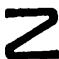
\includegraphics[keepaspectratio]{images/part003_6b42bd98.jpg}}

Let A be the ring of v. If v is discrete, Proposition 8 of §3, no. 6 shows that the topology induced by \(T_{v}\) on A is the m(A)-adic topology. This is not so in general (Exercise 4).

PROPOSITION 2. Let K be a not necessarily commutative field, v a non-improper valuation on K, A the ring of v and m the ideal of v. For K with the topology \(\mathcal{T}_v\) to be locally compact, it is necessary and sufficient that the following conditions be fulfilled:

\begin{enumerate}
\def\labelenumi{(\roman{enumi})}
\item
  K is complete;
\item
  v is discrete;
\item
  the residue field \(\kappa(A)\) is finite.
\end{enumerate}

If so, A is compact.

Suppose K is locally compact. Then it is complete (General Topology, Chapter III, § 3, no. 3, Corollary 1 to Proposition 4); further there exists a compact neighbourhood of 0, which contains a neighbourhood \(\mathbf{V}_{\alpha}^{\prime}\) , where \(\alpha\) belongs to the value group of \(v\) ; in other words, there exists \(a \neq 0\) in \(\mathbf{K}^*\) such that A.a is compact and it follows that \(\mathrm{A} = (\mathrm{A}.a)a^{-1}\) is compact. As every ideal \(\mathfrak{b} \neq (0)\) of A is open, A/b is compact and discrete (General Topology, Chapter III, § 2, no. 5, Proposition 14) and therefore finite and in particular \(\kappa(\mathrm{A}) = \mathrm{A}/\mathfrak{m}\) is finite. Moreover, for \(y \neq 0\) in \(\mathfrak{m}\) , the ring A/Ay being finite, there is only a finite number of ideals of A containing Ay and the set P of elements of the form \(v(x)\) such that

\[
0 <   v (x) \leqslant v (y)
\]

is finite; as \(v(\mathbf{K}^{*})\) is totally ordered, P has a least element \(\gamma\) . Then for all \(x \in A\) such that \(v(x) > 0\) , either \(v(x) > v(y) \geqslant \gamma\) , or \(v(x) \leqslant v(y)\) and then \(v(x) \geqslant \gamma\) by definition, so that \(\gamma\) is the least of the elements >0 of \(v(\mathbf{K}^{*})\) . As P is finite, there is a greatest integer \(m \geqslant 0\) such that \(m_{\gamma} \in P\) , whence \(m\gamma \leqslant v(y) < (m + 1)\gamma.\) We deduce that \(0 \leqslant v(y) - m\gamma < \gamma\) and by definition of \(\gamma\) this implies \(v(y) = m\gamma.\) Therefore \(v(\mathbf{K}^{*}) = \mathbf{Z}. \gamma\) and the valuation \(v\) is discrete.

Conversely, suppose conditions (i), (ii), (iii) hold. We may restrict our attention to the case where v is normed; let u be a uniformizer for v. Then \(\kappa(\mathbf{A}) = \mathbf{A}/\mathbf{A}u\) and hence A/Au is finite. As \(x \mapsto xu^{n}\) defines by taking quotients an isomorphism of the additive group A/Au onto \(Au^{n}/Au^{n+1}\) , \(A/Au^{j}\) is finite for all \(j \geqslant 0\) . As A is closed in K, it is complete and hence isomorphic to the inverse limit of the \(A/Au^{j}\) (General Topology, Chapter III, §7, no. 3, Proposition 2) and therefore compact. Since A is open in K, it is therefore seen that K is locally compact.

Remark. Note that it is sufficient in this proof to suppose that A is complete.

We shall see in § 9 that a field K fulfilling the conditions of Proposition 2 admits a centre which is either a finite algebraic extension of a p-adic field, or a field \(\mathbf{F}_{q}((\mathbf{T}))\) of formal power series over a finite field; moreover K is of finite rank over its centre.

\subsection{Topological vector spaces over a field with a valuation}

Throughout let K be a (not necessarily commutative) field, v a valuation on K and G its order group. K is given the topology \(T_{v}\) .

PROPOSITION 3. Let E be a left topological vector space over K which is Hausdorff and of dimension 1. Suppose that v is not improper. For all \(x_{0} \neq 0\) in E, the mapping \(a \mapsto ax_{0}\) of \(K_{s}\) onto E is a topological isomorphism.

This mapping is a continuous algebraic isomorphism. It is sufficient to show that it is bicontinuous. Let \(\alpha \in \mathbf{G}\) . We need to show that there exists a neighbourhood V of 0 in E such that the relation \(ax_0 \in \mathbf{V}\) implies \(v(a) > \alpha\) . Let \(a_0 \in \mathbf{K}^*\) be such that \(v(a_0) = \alpha\) . As E is Hausdorff, there exists a neighbourhood W of 0 in E such that \(a_0 x_0 \notin \mathbf{W}\) . As \(v\) is not improper, there exist a neighbourhood W' of 0 in E and an element \(\beta\) of G such that the relations \(y \in \mathbf{W}'\) , \(v(a) \geqslant \beta\) imply \(ay \in \mathbf{W}\) . Let \(a_1 \in \mathbf{K}^*\) be such that \(v(a_1) = -\beta\) . The relations \(ax_0 \in a_1^{-1} \mathbf{W}'\) and \(v(a) \leqslant \alpha\) imply \(a_1 ax_0 \in \mathbf{W}'\) and \(v(a_0 a^{-1} a_1^{-1}) = \alpha + \beta - v(a) \geqslant \beta\) and hence \(a_0 x_0 = a_0 a^{-1} a_1^{-1}(a_1 ax_0) \in \mathbf{W}\) , which is absurd; in other words, the relation \(ax_0 \in a_1^{-1} \mathbf{W}\) implies \(v(a) > \alpha\) .

COROLLARY. Let E be a left topological vector space over K, H a closed hyperplane of E and D a 1-dimensional vector subspace of E an algebraic supplement of H. Suppose that v is not improper. Then D is a topological supplement of H.

Taking account of Propositions 1 and 3, the proof is the same as that of Topological Vector Spaces, Chapter I, § 2, Corollary 2 to Theorem 1.

PROPOSITION 4. Suppose that \(v\) is not improper and \(K\) is complete. Let \(E\) be a left topological vector space over \(K\) , which is Hausdorff and of finite dimension \(n\) . For every basis \((e_i)_{1 \leqslant i \leqslant n}\) of \(E\) over \(K\) , the mapping \((a_i) \mapsto \sum_{i=1}^{n} a_i e_i\) of \(K_s^n\) onto \(E\) is a topological vector space isomorphism.

Taking account of Proposition 3 and its corollary, the proof is the same as that of Topological Vector Spaces, Chapter I, § 2, Theorem 2.

COROLLARY. Suppose that v is not improper and K is complete. Let E be a Hausdorff topological vector space over K and F a finite-dimensional vector subspace of E. Then F is closed.

F is complete.

\subsection{The completion of a field with a valuation}

PROPOSITION 5. Let K be a not necessarily commutative field, v a valuation on K and G the group \(v(\mathbf{K}^{*})\) with the discrete topology.

\begin{enumerate}
\def\labelenumi{(\alph{enumi})}
\item
  The completion ring \(\hat{\mathbf{K}}\) of \(\mathbf{K}\) (with \(\mathcal{T}_v\) ) is a topological field.
\item
  The mapping \(v: \mathbf{K}^* \to \mathbf{G}\) can be extended uniquely to a continuous mapping \(\hat{v}: \hat{\mathbf{K}}^* \to \mathbf{G}\) . The mapping \(\hat{v}\) (extended by \(\hat{v}(0) = +\infty\) ) is a valuation on \(\hat{\mathbf{K}}\) and \(\hat{v}(\hat{\mathbf{K}}^*) = v(\mathbf{K}^*)\) .
\item
  The topology on \(\hat{\mathbf{K}}\) is the topology defined by the valuation \(\hat{v}\) .
\item
  For all \(\alpha \in \mathbf{G}\) let \(\mathrm{V}_{\alpha}, \mathrm{V}_{\alpha}'\) be the subgroups of \(\mathbf{K}\) defined by the conditions \(v(x) > \alpha\) , \(v(x) \geqslant \alpha\) . Then the closures \(\overline{\mathrm{V}}_{\alpha}, \overline{\mathrm{V}}_{\alpha}'\) of \(\mathrm{V}_{\alpha}, \mathrm{V}_{\alpha}'\) in \(\hat{\mathbf{K}}\) are defined by the conditions \(\hat{v}(x) > \alpha\) , \(\hat{v}(x) \geqslant \alpha\) respectively.
\item
  The ring of \(\hat{v}\) is the completion \(\hat{\mathbf{A}}\) of the ring \(\mathbf{A}\) of \(v\) ; the ideal of \(\hat{v}\) is the completion \(\hat{\mathfrak{m}}\) of the ideal \(\mathfrak{m}\) of \(v\) .
\item
  \(\hat{\mathbf{A}} = \mathbf{A} + \hat{\mathfrak{m}}\) ; the residue field of \(\hat{v}\) is canonically identified with that of \(v\) .
\end{enumerate}

To prove (a) it suffices (General Topology, Chapter III, § 6, no. 8, Proposition 7) to show the following: let \(\mathfrak{F}\) be a Cauchy filter (with respect to the additive uniform structure) on \(\mathbf{K}^*\) for which 0 is not a cluster point; then the image of \(\mathfrak{F}\) under the bijection \(x \mapsto x^{-1}\) is a Cauchy filter (with respect to the additive uniform structure). For since 0 is not a cluster point of \(\mathfrak{F}\) , there exists \(\mathbf{M} \in \mathfrak{F}\) and \(\beta \in \mathbf{G}\) such that \(\beta\) is an upper bound of \(v(\mathbf{M})\) . Let \(\alpha \in \mathbf{G}\) . If \(\mathbf{M}'\) is an element of \(\mathfrak{F}\) contained in \(\mathbf{M}\) and such that \(v(x - y) > \sup (\alpha + 2\beta, \beta)\) for \(x \in \mathbf{M}'\) and \(y \in \mathbf{M}'\) , then \(v(x^{-1} - y^{-1}) > \alpha\) for \(x \in \mathbf{M}'\) and \(y \in \mathbf{M}'\) (no. 1, Lemma 1). Whence (a).

By Proposition 1 of no. 1, \(v|K^*\) is a continuous homomorphism from \(K^*\) to \(G\) and hence can be extended uniquely to a continuous homomorphism \(\hat{v}\) from \(K^*\) to \(G\) . the Relation

\[
\hat {v} (x + y) \geqslant \inf (\hat {v} (x), \hat {v} (y))
\]

holds in \(\mathbf{K}^*\) and hence also holds in \(\hat{\mathbf{K}}^*\) by continuity. Thus \(\vartheta\) (extended by \(\hat{\upsilon}(0) = +\infty\) ) is a valuation on \(\hat{\mathbf{K}}\) and (b) is proved.

We now show (d). Let \(\alpha \in G\) and \(x \in \overline{V}_{\alpha} - \{0\}\) . For \(y\) in \(V_{\alpha}\) sufficiently close to \(x\) , \(\hat{v}(x) = \hat{v}(y) = v(y)\) and hence \(\hat{v}(x) > \alpha\) . Conversely, let \(x \in \widehat{K}^*\) be such that \(\hat{v}(x) > \alpha\) ; for \(y\) in \(K^*\) sufficiently close to \(x\) , \(v(y) = \hat{v}(y) = \hat{v}(x)\) and therefore \(y \in V_{\alpha}\) , whence \(x \in \overline{V}_{\alpha}\) . Thus \(\overline{V}_{\alpha}\) is the set of \(x \in \widehat{K}\) such that \(\hat{v}(x) > \alpha\) . The argument is analogous for \(V_{\alpha}'\) . This proves (d).

Taking account of Proposition 7 of General Topology, Chapter III, § 3, no. 4, assertion (c) is a consequence of (d). Assertion (e) is a special case of (d). Finally let \(x \in \hat{\mathbf{A}}\) ; there exists \(y \in \mathbf{A}\) such that \(\hat{v}(x - y) > 0\) ; then \(z = x - y \in \hat{\mathfrak{m}}\) and hence \(x = y + z \in \mathbf{A} + \hat{\mathfrak{m}}\) ; thus \(\hat{\mathbf{A}} = \mathbf{A} + \hat{\mathfrak{m}}\) , which shows (f).

Remark. For all \(x \in \hat{\mathbf{K}}\) not belonging to \(\hat{\mathbf{A}}\) , there exists \(x_0 \in \mathbf{K}\) such that \(\hat{v}(x - x_0) > 0\) , \(\hat{v}(x) = \hat{v}(x_0) = v(x_0) < 0\) ; then \(x_0^{-1}x \in \hat{\mathbf{A}}\) and, as \(x_0^{-1} \in \mathbf{A}\) , it is seen that, if we set \(S = A - \{0\}\) , it is possible to write \(\hat{\mathbf{K}} = S^{-1}\hat{\mathbf{A}}\) .

\section{ABSOLUTE VALUES}

\subsection{Preliminaries on absolute values}

Let K be a field (commutative or not). Recall (General Topology, Chapter IX, §3, no. 2, Definition 2) that an absolute value on K is any mapping f from K to \(R_{+}\) satisfying the following axioms:

\((\mathrm{VA}_{\mathbf{I}})\) The relation \(f(x) = 0\) is equivalent to \(x = 0\) .

\((\mathrm{VA}_{\mathrm{II}}) f(xy) = f(x)f(y)\) for all \(x, y\) in \(\mathbf{K}\) .

\((\mathrm{VA}_{\mathrm{III}}) f(x + y) \leqslant f(x) + f(y)\) for all \(x, y\) in \(\mathbf{K}\) .

It follows from \((\mathrm{VA}_{\mathbf{I}})\) and \((\mathrm{VA}_{\mathbf{II}})\) that \(f(1) = 1, f(-1) = 1\) and

\[
f (x ^ {- 1}) = \frac {1}{f (x)}
\]

for \(x \neq 0\) .

For a mapping \(f\) from \(\mathbf{K}\) to \(\mathbf{R}_{+}\) and a real number \(\mathbf{A} > 0\) , let \((\mathrm{U}_{\mathbf{A}})\) denote the relation

\[
f (x + y) \leqslant \mathrm{A}. \sup (f (x), f (y)) \quad \text {   for   all   } x, y \text {   in   } \mathrm{K}.
\]

We shall denote by \(\mathcal{V}(\mathbf{K})\) the set of mappings \(f\) from \(\mathbf{K}\) to \(\mathbf{R}_{+}\) satisfying \((\mathrm{VA}_{\mathbf{I}})\) and \((\mathrm{VA}_{\mathbf{II}})\) and for which there exists an \(\mathbf{A} > 0\) (depending on \(f\) ) such that \((\mathbf{U}_{\mathbf{A}})\) holds.

Note that if \(f \in \mathcal{V}(\mathbf{K})\) , then, putting \(x = 1, y = 0\) in \((\mathrm{U}_{\mathbf{A}})\) ,

\[
1 = f (1) \leqslant A. \sup (f (1), f (0)) = A.
\]

PROPOSITION 1. For a mapping \(f\) from \(\mathbf{K}\) to \(\mathbf{R}_+\) satisfying \((\mathrm{VA}_{\mathbf{I}})\) and \((\mathrm{VA}_{\mathbf{II}})\) to belong to \(\mathcal{V}(\mathbf{K})\) , it is necessary and sufficient that \(f(1 + x)\) be bounded in the set of \(x \in \mathbf{K}\) such that \(f(x) \leqslant 1\) .

If \(f\) satisfies \((\mathrm{U}_{\mathbf{A}})\) , then \(f(1 + x) \leqslant \mathbf{A}\) if \(f(x) \leqslant 1\) . Conversely, suppose that \(f(x + 1) \leqslant \mathbf{A}\) for the \(x \in \mathbf{K}\) such that \(f(x) \leqslant 1\) (which implies that \(\mathbf{A} \geqslant f(1) = 1\) ); then, if \(x = 0\) or \(y = 0\) , condition \((\mathrm{U}_{\mathbf{A}})\) is fulfilled; if on the other hand \(x \neq 0\) and \(y \neq 0\) , we may assume for example that \(f(y) \leqslant f(x)\) , hence, by \((\mathrm{VA}_{\mathrm{II}}), f(yx^{-1}) \leqslant 1\) and therefore \(f(1 + yx^{-1}) \leqslant \mathbf{A}\) , which gives, by virtue of \((\mathrm{VA}_{\mathrm{II}}), f(x + y)f(x)^{-1} \leqslant \mathbf{A}\) ; whence

\[
f (x + y) \leqslant A f (x) \leqslant A. \sup (f (x), f (y)).
\]

If \(f\) is an absolute value on \(\mathbf{K}\) , then \(f(n,1) \leqslant n\) by induction on the integer \(n > 0\) starting from \((\mathrm{VA}_{\mathrm{III}})\) ; conversely:

PROPOSITION 2. Let \(f\) be a mapping of \(\mathbf{K}\) to \(\mathbf{R}_+\) belonging to \(\mathcal{V}(\mathbf{K})\) ; if there exists \(\mathbf{C} > 0\) such that \(f(n,1) \leqslant \mathbf{C}.n\) for every integer \(n > 0\) , \(f\) is an absolute value on \(\mathbf{K}\) .

By induction on r > 0 we deduce from \((\mathbf{U}_{\mathbf{A}})\) the relation

\[
f (x _ {1} + x _ {2} + \dots + x _ {2 ^ {r}}) \leqslant A ^ {r} \sup _ {1 \leqslant i \leqslant 2 ^ {r}} f (x _ {i})\tag{1}
\]

for every family \((x_{i})\) of \(2^{r}\) elements of \(\mathbf{K}\) . We set \(n = 2^{r} - 1\) ; for all \(x \in \mathbf{K}\) , we deduce from (1)

\[
(f (1 + x)) ^ {n} = f ((1 + x) ^ {n}) = f \left(\sum_ {i = 0} ^ {n} \binom {n} {i} x ^ {i}\right) \leqslant A ^ {r} \sup \left(f \left(\binom {n} {i}\right) (f (x)) ^ {i}\right)
\]

\[
\leqslant \mathrm{CA} ^ {r} \sum_ {i = 0} ^ {n} \binom {n} {i} (f (x)) ^ {i} = \mathrm{CA} ^ {r} (1 + f (x)) ^ {n}
\]

for \(f\left(\binom{n}{i}\right) \leqslant C\binom{n}{i}\) ; therefore

\[
f (1 + x) \leqslant \mathrm{C} ^ {1 / n} \mathrm{A} ^ {r / n} (1 + f (x)).
\]

Letting r tend to \(+\infty\) , we obtain \(f(1+x)\leqslant1+f(x)\) for all \(x\in K\) ; applying this inequality with x replaced by \(xy^{-1}\) (where \(y\neq0\) ) and taking account of \((\mathrm{VA}_{\mathrm{II}})\) , we obtain relation \((\mathrm{VA}_{\mathrm{III}})\) , which proves the proposition.

COROLLARY 1. For a mapping f from K to \(R_{+}\) to be an absolute value, it is necessary and sufficient that it satisfy conditions (VA \(_{I}\) ), (VA \(_{II}\) ) and (U \(_{2}\) ).

It is necessary, for \((\mathrm{VA}_{\mathrm{II}})\) implies

\[
f (x + y) \leqslant f (x) + f (y) \leqslant 2 \sup (f (x), f (y)).
\]

Conversely, suppose \(f\) satisfies \((\mathrm{VA}_{\mathrm{I}}), (\mathrm{VA}_{\mathrm{II}})\) and \((\mathrm{U}_2)\) ; for every integer \(n > 0\) , let \(r\) be the least integer such that \(2^r \geqslant n\) ; if in (1) A is replaced by 2, the \(x_i\) of index \(i \leqslant n\) by 1 and the \(x_i\) of index \(i > n\) by 0, we obtain

\[
f (n. 1) \leqslant 2 ^ {r} <   2 n;
\]

then Proposition 2 may be applied with \(\mathbf{C} = 2\) and hence \(f\) is an absolute value.

COROLLARY 2. For a mapping \(f\) of \(\mathbf{K}\) to \(\mathbf{R}_+\) to belong to \(\mathcal{V}(\mathbf{K})\) , it is necessary and sufficient that it be of the form \(g^t\) , where \(t > 0\) and \(g\) is an absolute value on \(\mathbf{K}\) .

To say that \(f\) satisfies \((\mathbf{U}_{\mathbf{A}})\) is equivalent to saying that \(f^s\) satisfies \((\mathbf{U}_{\mathbf{A}^s})\) ; as there exists \(s > 0\) such that \(\mathbf{A}^s \leqslant 2\) , Corollary 1 shows that for such a value of \(s, f^s\) is an absolute value.

\subsection{Ultrametric absolute values}

A mapping f of K to \(R_{+}\) is called an ultrametric absolute value if it satisfies conditions ( \(VA_{I}\) ), ( \(VA_{II}\) ) and ( \(U_{1}\) ) (which obviously implies that f is an absolute value).

PROPOSITION 3. Let \(f\) be a mapping of \(\mathbf{K}\) to \(\mathbf{R}_+\) . The following properties are equivalent:

\begin{enumerate}
\def\labelenumi{(\alph{enumi})}
\item
  \(f\) is an ultrametric absolute value.
\item
  There exists a valuation \(v\) on \(\mathbf{K}\) with values in \(\mathbf{R}\) and a real number \(a\) such that \(0 < a < 1\) and \(f = a^v\) .
\item
  \(f\) belongs to \(\mathcal{V}(\mathbf{K})\) and \(f(n,1) \leqslant 1\) for every integer \(n > 0\) .
\item
  For all \(s > 0, f^s\) is an absolute value.
\end{enumerate}

For every real number \(c\) such that \(0 < c < 1\) , the mapping \(t \mapsto c^t\) is an isomorphism of the ordered group \(\mathbf{R}\) (with the opposite ordering to the usual ordering) on the ordered group \(\mathbf{R}_+^*\) ; this shows the equivalence of (a) and (b). Clearly (a) implies (c); (c) implies (d), for we deduce from (c) that

\[
(f (n. 1)) ^ {s} \leqslant 1 \leqslant n
\]

for every integer \(n > 0\) and Proposition 2 of no. 1 shows that \(f^s\) is an absolute value. Finally (d) implies (a): for if \(f^s\) is an absolute value, it satisfies \((\mathbf{U}_2)\) and hence \(f\) satisfies \((\mathbf{U}_{2^{1 / s}})\) for all \(s > 0\) and therefore also \((\mathbf{U}_1)\) , letting \(s\) tend to \(+\infty\) .

COROLLARY. If K is a (not necessarily commutative) field of characteristic p > 0, every function on \(\mathcal{V}(\mathbf{K})\) is an ultrametric absolute value.

Every non-zero element \(z = n.1\) ( \(n\) an integer \(>0\) ) belongs to the prime subfield \(\mathbf{F}_p\) of \(K\) and hence satisfies the relation \(z^{p-1} = 1\) , which implies \(f(z) = 1\) and we may apply Proposition 3 (c).

Given a real number \(c\) such that \(0 < c < 1\) , the formulae

\[
f (x) = c ^ {v (x)}, \quad v (x) = \log_ {c} f (x)
\]

therefore establish a one-to-one correspondence between ultrametric absolute values on K and valuations on K with real values. The improper valuation corresponds to the improper absolute value (General Topology, Chapter IX, § 3, no. 2). Let \(v_{1}, v_{2}\) be two valuations on K with real values and \(f_{1}, f_{2}\) the corresponding absolute values; for \(v_{1}\) and \(v_{2}\) to be equivalent, it is necessary and sufficient that \(f_{1}\) and \(f_{2}\) be so: for to say that \(v_{1}\) and \(v_{2}\) are equivalent amounts to saying that the relations \(v_{1}(x) \geqslant 0\) and \(v_{2}(x) \geqslant 0\) are equivalent or again that the relations \(f_{1}(x) \leqslant 1\) and \(f_{2}(x) \leqslant 1\) are equivalent; it is therefore sufficient to apply Proposition 5 of General Topology, Chapter IX, §3, no. 2. Moreover (loc. cit.) for the topologies defined on K by \(f_{1}\) and \(f_{2}\) to be identical, it is necessary and sufficient that \(f_{1}\) and \(f_{2}\) be equivalent.

\subsection{Absolute values on Q}

PROPOSITION 4. Let \(f\) be a mapping of \(\mathbf{Q}\) to \(\mathbf{R}_+\) belonging to \(\mathcal{V}(\mathbf{Q})\) . Then:

\begin{enumerate}
\def\labelenumi{(\roman{enumi})}
\item
  Either \(f\) is the improper absolute value on \(\mathbf{Q}\) .
\item
  Or there exists a real number \(a\) and a prime number \(p\) such that \(0 < a < 1\) and \(f = a^{v_p}\) , where \(v_p\) is the \(p\) -adic valuation.
\item
  Or there exists \(s > 0\) such that \(f(x) = |x|^s\) for all \(x \in \mathbf{Q}\) .
\end{enumerate}

In case (iii) for \(f\) to be an absolute value on \(\mathbf{Q}\) , it is necessary and sufficient that \(0 < s \leqslant 1\) .

Suppose first that \(f(n) \leqslant 1\) for every integer \(n > 0\) . By Proposition 3 of no. 2 there exist a real number \(b\) and a valuation \(v\) on \(\mathbf{Q}\) such that \(0 < b < 1\) and \(f = b^v\) . Now, we know (§ 3, no. 4, Example 4) that the only valuations on \(\mathbf{Q}\) are (up to equivalence) the improper valuation and the \(p\) -adic valuations \(v_p\) ; we therefore have either case (i) or case (ii).

Suppose from now on that there exists an integer \(h > 0\) such that \(f(h) > 1\) ; by no. 1, Corollary 2 to Proposition 2, there exists a number \(\rho > 0\) such that \(f^{\rho}\) is an absolute value; let us write

\[
g (x) = \rho \log (f (x)) / \log | x |
\]

for every rational number \(x \neq 0\) . Let \(a, b\) be two integers \(\geqslant 2\) ; for every integer \(n \geqslant 2\) let \(q(n)\) denote the integral part of \(n\) . log \(a / \log b\) , in other words the least integer \(m\) such that \(a^n < b^{m+1}\) ; the expansion of \(a^n\) to base \(b\) is therefore

\[
a ^ {n} = c _ {0} + c _ {1} b + \dots + c _ {q (n)} b ^ {q (n)}\tag{2}
\]

where \(0 \leqslant c_{i} < b\) for \(0 \leqslant i \leqslant q(n)\) . As \(f^{\rho}\) is an absolute value, \(f^{\rho}(c_{i}) \leqslant c_{i} \leqslant b\) and we therefore deduce from (2) that

\[
\begin{array}{r l} (f (a)) ^ {n \rho} = (f (a ^ {n})) ^ {\rho} & \leqslant b (1 + (f (b)) ^ {\rho} + \dots + (f (b)) ^ {\rho q (n)}) \\ & \leqslant b (q (n) + 1) (\sup (1, (f (b)) ^ {\rho})) ^ {q (n)}. \end{array}
\]

Taking logarithms on both sides of this inequality and dividing by \(n.\log a\) , we obtain

\[
g (a) \leqslant \frac {\log b}{n . \log a} + \frac {\log (q (n) + 1)}{q (n)} \cdot \frac {q (n)}{n . \log a} + \frac {\sup (0 , \rho \log f (b))}{\log a} \cdot \frac {q (n)}{n}.\tag{3}
\]

Note now that as \(n\) tends to \(+\infty\) , \(q(n) / n\) tends to \(\log a / \log b\) ; therefore \(q(n)\) tends to \(+\infty\) and

\[
\log (q (n) + 1) / q (n)
\]

tends to 0 (Functions of a Real Variable, Chapter III, § 2, no. 1). Taking the limit in (3), we obtain

\[
g (a) \leqslant \frac {\sup (0 , \rho \log f (b))}{\log b} = \sup (0, g (b)).\tag{4}
\]

But \(f(h) > 1\) , whence \(g(h) > 0\) ; if \(a\) is replaced by \(h\) in (4), we obtain \(\sup(0, g(b)) > 0\) and hence

\[
\sup (0, g (b)) = g (b).
\]

Then, for any integers \(a\) , \(b\) at least equal to 2, \(g(a) \leqslant g(b)\) and therefore \(g(a) = g(b)\) , exchanging the roles of \(a\) and \(b\) . In other words, there exists a constant \(\lambda\) such that \(g(a) = \lambda\) for every integer \(a \geqslant 2\) ; if we write \(s = \lambda / \rho\) , then \(f(a) = |a|^s\) for every integer \(a \geqslant 2\) . As \(f(xy) = f(x)f(y)\) and \(f(-x) = f(x) = |x|^s\) for all \(x \in \mathbf{Q}\) . Finally, if \(0 < s \leqslant 1\) , we know that \(x \mapsto |x|^s\) is an absolute value (General Topology, Chapter IX, §3, no. 2); conversely, if \(s\) is such that \(x \mapsto |x|^s\) is an absolute value on \(\mathbf{Q}\) , then \((1 + 1)^s \leqslant 1^s + 1^s\) , that is \(2^s \leqslant 2\) , whence \(s \leqslant 1\) .

\subsection{Structure of fields with a non-ultrametric absolute value}

THEOREM 1 (Gelfand-Mazur). Let \(\mathbf{K}\) be an algebra over the field \(\mathbf{R}\) with the two following properties:

\begin{enumerate}
\def\labelenumi{(\arabic{enumi})}
\item
  K is a (not necessarily commutative) field.
\item
  There exists on K a norm \(x \mapsto \| x \|\) compatible with the algebra structure on K (General Topology, Chapter IX, § 3, no. 7, Definition 9).
\end{enumerate}

Then the algebra \(\mathbf{K}\) is isomorphic to one of the algebras \(\mathbf{R},\mathbf{C}\) or \(\mathbf{H}\) .

Recall (loc. cit.) that it may always be assumed that \(\|xy\|\leqslant\|x\|. \|y\|\) for all x,y in K. We shall give K the topology (compatible with the algebra structure) defined by the norm.

\textbf{(A) First case: \(\mathbf{K}\) is commutative and there exists \(j\in \mathbf{K}\) such that \(j^2 = -1\)}\par

Then there exists an isomorphism \(\sigma\) of the field \(\mathbf{C}\) onto a subfield of \(\mathbf{K}\) such that \(\sigma(\xi + i\eta) = \xi \cdot 1 + \eta \cdot j\) for \(\xi, \eta\) in \(\mathbf{R}\) . We shall prove by reductio ad absurdum that \(\mathbf{K} = \sigma(\mathbf{C})\) . Suppose then that there exists \(x \in \mathbf{K} - \sigma(\mathbf{C})\) ; for all \(z \in \mathbf{C}, x - \sigma(z)\) is therefore invertible in \(\mathbf{K}\) ; let us write \(\mathrm{F}(z) = (x - \sigma(z))^{-1}\) ; as \(\sigma\) is continuous and the inverse is continuous on \(\mathbf{K}\) (General Topology, Chapter IX, §3, no. 7, Proposition 13 applied to the completion algebra of \(\mathbf{K}\) ), \(\mathbf{F}\) is a continuous mapping of \(\mathbf{C}\) to \(\mathbf{K}\) . Moreover, we may write for \(z \neq 0\)

\[
\mathrm{F} (z) = (\sigma (z)) ^ {- 1} (x (\sigma (z)) ^ {- 1} - 1) ^ {- 1}.
\]

But, as \((\sigma(z))^{-1} = \sigma(z^{-1})\) tends to 0 as \(z\) tends to infinity in \(\mathbf{C}\) , it is seen that \(\mathbf{F}(z)\) tends to 0; in other words, \(z \mapsto \| \mathbf{F}(z) \|\) is a continuous real-valued function, \(\geqslant 0\) on \(\mathbf{C}\) , tending to 0 at the point at infinity and which can therefore be considered as a continuous function on the compact space \(\tilde{\mathbf{C}}\) obtained by adjoining to \(\mathbf{C}\) a point at infinity. The least upper bound \(\alpha\) of \(\| \mathbf{F} \|\) on \(\mathbf{C}\) is therefore finite and \(>0\) and the set \(\mathrm{P}\) of complex numbers \(z\) such that \(\| \mathrm{F}(z) \| = \alpha\) is closed and non-empty (General Topology, Chapter IV, §6, no. 1, Theorem 1).

Let \(z \in \mathbf{P}\) ; let us write \(y = x - \sigma(z)\) and let \(t\) be a complex number \(\neq 0\) such that \(\| \sigma(t) \| < \alpha^{-1}\) , whence \(\| \sigma(t).y^{-1} \| < 1\) by definition of \(\alpha\) . The sequence of the \((\sigma(t)y^{-1})^n\) and that of the \(n(\sigma(t)y^{-1})^n\) therefore tend to 0 in \(K\) as \(n\) tends to \(+\infty\) , for so do the corresponding sequences of norms in \(R\) . On the other hand note that for every polynomial \(\mathbf{H}(\mathbf{T}) = \prod_{k=1}^{p} (\mathbf{T} - \sigma(c_k))\) , where the \(c_k\) are distinct complex numbers, in the field \(\mathbf{K}(\mathbf{T})\) of rational functions

\[
\frac {\mathrm{H} ^ {\prime} (\mathrm{T})}{\mathrm{H} (\mathrm{T})} = \sum_ {k = 1} ^ {p} \frac {1}{\mathrm{T} - \sigma (c _ {k})}.\tag{5}
\]

We apply this formula to the polynomial

\[
\mathrm{H} (\mathrm{T}) = \mathrm{T} ^ {n} - (\sigma (t)) ^ {n} = \prod_ {k = 0} ^ {n - 1} \left(\mathrm{T} - \sigma \left(\omega_ {n} ^ {k} t\right)\right),
\]

where \(\omega_{n}=\exp(2\pi i/n)\) , and substitute for T the element \(y\in K\) , which is distinct from all the \(\sigma(\omega_{n}^{k}t)\) . It follows (in the commutative field K) that

\[
\frac {n y ^ {n - 1}}{y ^ {n} - (\sigma (t)) ^ {n}} = \frac {1}{y - \sigma (t)} + \sum_ {k = 1} ^ {n - 1} \frac {1}{y - \sigma \left(\omega_ {n} ^ {k} t\right)}.\tag{6}
\]

Taking account of the definitions of F and y, we obtain

\[
\begin{array}{r l} \mathrm{F} (z + t) + \sum_ {k = 1} ^ {n - 1} \mathrm{F} (z + \omega_ {n} ^ {k} t) - n \mathrm{F} (z) & \\ = \frac {n y ^ {n - 1}}{y ^ {n} - (\sigma (t)) ^ {n}} - \frac {n}{y} = \frac {1}{y} \cdot \frac {n (\sigma (t) y ^ {- 1}) ^ {n}}{1 - (\sigma (t) y ^ {- 1}) ^ {n}}. \end{array}\tag{7}
\]

But by virtue of the choice of t and the remarks made above, the last expression in (7) tends to 0 as n tends to \(+\infty\) ; hence

\[
\| \mathrm{F} (z + t) \| = \lim _ {n \to + \infty} \| n \mathrm{F} (z) - \sum_ {k = 1} ^ {n - 1} \mathrm{F} (z + \omega_ {n} ^ {k} t) \|.\tag{8}
\]

Now, \(\| \mathrm{F}(z)\| = \alpha\) and \(\| \mathrm{F}(z + \omega_n^kt)\| \leqslant \alpha\) by definition of \(\alpha\) , whence

\[
\left\| n \mathrm{F} (z) - \sum_ {k = 1} ^ {n - 1} \mathrm{F} (z + \omega_ {n} ^ {k} t) \right\| \geqslant
\]

\[
n \| \mathrm{F} (z) \| - \sum_ {k = 1} ^ {n - 1} \| \mathrm{F} (z + \omega_ {n} ^ {k} t) \| \geqslant n \alpha - (n - 1) \alpha = \alpha .
\]

Therefore by (8), letting \(n\) tend to \(+\infty\) , \(\| \mathbf{F}(z + t) \| \geqslant \alpha\) and by definition of \(\alpha\) this implies

\[
\| \mathrm{F} (z + t) \| = \alpha ,
\]

in other words \(z + t \in P\) . This proves that the set P is open in C; as it is also closed and non-empty and C is connected, P = C and \(\|F\|\) is therefore constant on C; as this function tends to 0 at the point at infinity, \(\|F(z)\| = 0\) in C and in particular \(\|F(0)\| = \|x^{-1}\| = 0\) , which is absurd.

\textbf{(B) Second case; \(\mathbf{K}\) is commutative and \(-1\) is not the square of an element of \(\mathbf{K}\)}\par

Let L be the commutative field obtained by adjoining to K a root j of \(T^{2} + 1\) ; L is a vector space over K admitting \((1, j)\) as a basis and L is obviously an algebra over R. Clearly the function \(x + yj \to \|x\| + \|y\|\) is a norm on L compatible with its structure as a vector space over R; on the other hand, for \(z = x + yj\) , \(z' = x' + y'j\) in L,

\[
\begin{array}{r l} \| z z ^ {\prime} \| & = \| x x ^ {\prime} - y y ^ {\prime} \| + \| x y ^ {\prime} + x ^ {\prime} y \| \leqslant \| x x ^ {\prime} \| + \| y y ^ {\prime} \| + \| x y ^ {\prime} \| + \| x ^ {\prime} y \| \\ & \leqslant \| x \| \cdot \| x ^ {\prime} \| + \| y \| \cdot \| y ^ {\prime} \| + \| x \| \cdot \| y ^ {\prime} \| + \| x ^ {\prime} \| \cdot \| y \| \\ & = (\| x \| + \| y \|) (\| x ^ {\prime} \| + \| y ^ {\prime} \|) = \| z \| \cdot \| z ^ {\prime} \|. \end{array}
\]

The norm thus defined is consequently compatible with the R-algebra structure on L. By case (A) L is an R-algebra isomorphic to C; now the only sub-R-algebra of C distinct from C is R and hence K is isomorphic to R.

\textbf{(C) Third case: K is not commutative}\par

Let Z be the centre of K and x an element of K not in Z; the subfield \(Z(x)\) of K is commutative and the norm induced by that on K is compatible with the R-algebra structure on \(Z(x)\) ; as \(Z \neq Z(x)\) and Z and \(Z(x)\) are R-algebras isomorphic to R or C by virtue of (A) and (B), Z is necessarily isomorphic to R and \(Z(x)\) to C. For all \(x \in K\) , \(Z(x)\) is therefore of rank \(\leqslant 2\) over Z. Now we have the following lemma:

LEMMA 1. Let D be a field with centre L such that, for all \(x \in \mathbf{D}\) , \(\mathbf{L}(x)\) is an extension of L of degree \(\leqslant m\) . Then the rank of D over L is \(\leqslant m^2\) .

We may obviously restrict our attention to the case where \(D \neq L\) . Then there exists in D a finite separable algebraic commutative extension E of L of degree >1 (Algebra, Chapter VIII, § 10, no. 3, Lemma 1); as \(E = L(x)\) for some suitable x in E (Algebra, Chapter V, § 7, no. 7, Proposition 12 and Chapter VII, § 5, no. 7), by hypothesis \([E: L] \leqslant m\) . Suppose the separable extension E is taken such that \([E: L]\) is finite and as great as possible and consider the centralizer \(E' \supset E\) of E in D, which is a field of centre E such that

\[
[ \mathbf {D} \colon \mathbf {E} ^ {\prime} ] = [ \mathbf {E} \colon \mathbf {L} ] \leqslant m
\]

(Algebra, Chapter VIII, § 10, no. 2, Theorem 2). If \(\mathbf{E} \neq \mathbf{E}'\) , there would exist in \(\mathbf{E}'\) a finite separable algebraic extension \(\mathbf{F}\) of \(\mathbf{E}\) of degree \(>1\) (Algebra, Chapter VIII, § 10, no. 3, Lemma 1); \(\mathbf{F}\) would therefore be a finite separable algebraic extension of \(\mathbf{L}\) (Algebra, Chapter V, § 7, no. 4, Proposition 7) of degree \(>[\mathrm{E:L}]\) , contrary to the definition of \(\mathbf{E}\) ; therefore \(\mathbf{E}' = \mathbf{E}\) , whence \([\mathrm{D:L}] = [\mathrm{D:E}][\mathrm{E:L}] \leqslant m^2\) .

Applying this lemma to K with m = 2, it is seen that K is a non-commutative extension field of R of finite rank and hence isomorphic to the field of quaternions H (Algebra, Chapter VIII, § 11, no. 2, Theorem 2).

Remark (1) We shall give in the chapter devoted to normed algebras a shorter proof of the Gelfand-Mazur Theorem which is valid for every Hausdorff locally convex topological algebra K over R and whose principle is the following: it is reduced (as in cases (B) and (C)) to the case where K is a commutative algebra over C; if \(x \in K - C.1\) , we consider as above the mapping \(z \mapsto (x - z.1)^{-1}\) of C to K, which is continuous and differentiable on C. For every element \(x'\) of the dual \(K'\) of the locally convex space K, \(z \mapsto \langle(x - z.1)^{-1}, x' \rangle\) is then a bounded integral function on C and therefore constant by Liouville's Theorem and we conclude as in part (A) of the proof of Theorem 1 that this necessarily implies \(\langle(x - z.1)^{-1}, x' \rangle = 0\) for all \(z \in C\) and all \(x' \in K'\) ; the Hahn-Banach Theorem shows that this conclusion is absurd, since \((x - z.1)^{-1} \neq 0\) . Note that the argument in part (A) of the proof of Theorem 1 differs from the above only in appearance, for this argument is only a special case of that which serves to prove the maximum principle for analytic functions, the summation over the roots of unity and passing to the limit being equivalent to calculating the integral \(\int_{\gamma} \frac{F(z + t) dt}{t}\) along a circle of centre 0 and the use of Cauchy's formula being avoided here, thanks to the particular form of the function F.

THEOREM 2 (Ostrowski). Let K be a (not necessarily commutative) field and f an element of \(\mathcal{V}(\mathbf{K})\) which is not an ultrametric absolute value. Then there exist a unique real number s > 0 and an isomorphism j of K onto an everywhere dense subfield of one of the fields R, C or H such that \(f(x) = |j(x)|^{s}\) for all \(x \in K (*)\) . For f to be an absolute value on K, it is necessary and sufficient that \(s \leqslant 1\) .

By no. 2, Corollary to Proposition 3, K is of characteristic 0 and hence an algebra over Q; for all \(x \in Q\) we write \(h(x) = f(x.1)\) ; clearly \(h \in \mathcal{V}(\mathbf{Q})\) and therefore Proposition 4 of no. 3 may be applied; neither of cases (i) and (ii) of the statement of this proposition can hold, for this would imply \(f(n.1) \leqslant 1\) for every integer n > 0 and f would be an ultrametric absolute value by virtue of no. 2, Proposition 3. Then there exists a real number \(s > 0\) such that \(h(x) = |x|^s\) for all \(x \in \mathbf{Q}\) , that is \(f(x,1) = |x|^s\) ; we write \(g = f^{1 / s}\) . Then \(g \in \mathcal{V}(\mathbf{K})\) and \(g(n,1) = n\) for every integer \(n\) ; Proposition 2 of no. 1 therefore shows that \(g\) is an absolute value on \(\mathbf{K}\) .

For \(x \in \mathbf{Q}\) and \(y \in \mathbf{K}\) , \(g(xy) = |x|g(y)\) and hence \(g\) is a norm on \(\mathbf{K}\) compatible with its \(\mathbf{Q}\) -algebra structure (with the usual absolute value on \(\mathbf{Q}\) ). The completion \(\hat{\mathbf{K}}\) of \(\mathbf{K}\) is therefore a normed algebra over \(\hat{\mathbf{Q}} = \mathbf{R}\) (General Topology, Chapter IX, § 3, no. 7); let \(\hat{g}\) be the norm on \(\hat{\mathbf{K}}\) the continuous extension of \(g\) . As \(g\) is an absolute value on \(\mathbf{K}\) , \(\hat{\mathbf{K}}\) is a field and \(\hat{g}\) an absolute value on \(\hat{\mathbf{K}}\) (General Topology, Chapter IX, § 3, no. 3, Proposition 6). By Theorem 1 there exists an \(\mathbf{R}\) -algebra isomorphism \(j\) of \(\hat{\mathbf{K}}\) onto one of the fields \(\mathbf{R}\) , \(\mathbf{C}\) or \(\mathbf{H}\) and \(g'(x) = |j(x)|\) is therefore an absolute value on \(\hat{\mathbf{K}}\) ; as \(\hat{\mathbf{K}}\) is finite-dimensional over \(\mathbf{R}\) and \(g'\) and \(\hat{g}\) coincide on the subfield \(\mathbf{R}\) . 1 of \(\hat{\mathbf{K}}\) , \(g' = \hat{g}\) by the following lemma:

LEMMA 2. Let L be a (not necessarily commutative) field and K a subfield of L such that L is a finite-dimensional left vector space over K. Let g be an absolute value on L and f its restriction to K. If K is complete and not discrete with respect to f, L is complete with respect to g; if further \(g'\) is another absolute value on L with the same restriction f to K, then \(g' = g\) .

As the topology defined by g is Hausdorff and compatible with the left vector K-space structure on L, the first assertion follows from Topological Vector Spaces, Chapter I, § 2, no. 3, Theorem 2. Moreover the topologies on L defined by g and \(g'\) are identical (loc. cit.); there therefore exists a real number s > 0 such that \(g' = g^{s}\) (General Topology, Chapter IX, § 3, no. 2, Proposition 5). Let x be an element of K such that \(f(x) \neq 1\) ; the equation \(g'(x) = g(x)\) proves that s = 1.

Returning to the proof of Theorem 2, it is seen that, if \(j\) denotes the restriction of \(\hat{j}\) to \(\mathbf{K}, j\) is an isomorphism of \(\mathbf{K}\) onto an everywhere dense subfield of \(\mathbf{R}\) , \(\mathbf{C}\) or \(\mathbf{H}\) and \(g(x) = |j(x)|\) for \(x \in \mathbf{K}\) , whence \(f(x) = |j(x)|^s\) .

Finally note that, if \(f\) is an absolute value on \(\mathbf{K}\) , \(h\) is an absolute value on \(\mathbf{Q}\) and \(s \leqslant 1\) by no. 3, Proposition 4; conversely, if \(s \leqslant 1\) , \(f = g^s\) is an absolute value on \(\mathbf{K}\) since \(g\) is (General Topology, Chapter IX, § 3, no. 2); this proves the last assertion of the statement.

\textbf{Remarks}\par

\begin{enumerate}
\def\labelenumi{(\arabic{enumi})}
\setcounter{enumi}{1}
\item
  If K is a field and a normed algebra over R, the norm is not necessarily an absolute value on K; for example, \(\xi + i\eta \to |\xi| + |\eta|\) is a norm on C compatible with its R-algebra structure.
\item
  For a proof of case (C) of Theorem 1 not using the general results of Algebra, Chapter VIII, see Exercise 2.
\end{enumerate}

\section{THE APPROXIMATION THEOREM}

\subsection{The intersection of a finite number of valuation rings}

PROPOSITION 1. Let K be a field, \((\mathbf{A}_{i})_{1 \leqslant i \leqslant n}\) a finite family of valuation rings of K and \(B = \bigcap_{i=1}^{n} A_{i}\) . We write \(p_{i} = B \cap m(A_{i})\) . Then \(A_{i} = B_{p_{i}}\) for all i and the field of fractions of B is K.

Clearly \(B_{p_t} \subset A_t\) . To prove the converse inclusion we need the following lemma: LEMMA 1. Let \(v_i (1 \leqslant i \leqslant n)\) be valuations on the field \(K\) and \(x \in K^*\) . Then there exists a polynomial \(f(X)\) of the form

\[
\begin{array}{l} (1) f (\mathbf {X}) = 1 + n _ {1} \mathbf {X} + \dots + n _ {k - 1} \mathbf {X} ^ {k - 1} + \mathbf {X} ^ {k} \\ \quad (k \geqslant 2, n _ {j} \in \mathbf {Z} for 1 \leqslant j \leqslant k - 1) \end{array}
\]

such that \(f(x) \neq 0\) and the element \(z = f(x)^{-1}\) enjoys the following properties for \(1 \leqslant i \leqslant n\) :

\[
\begin{array}{l l} v _ {i} (z) = 0 & \text { if } \quad v _ {i} (x) \geqslant 0 \\ v _ {i} (z) + v _ {i} (x) > 0 & \text { if } \quad v _ {i} (x) <   0. \end{array}
\]

Assuming this lemma for a moment, we show how it implies that \(A_{1} \subset B_{p_{1}}\) . Let x be a non-zero element of \(A_{1}\) . We apply the lemma to x and valuations \(v_{i}\) associated with the \(A_{i}\) . Then \(v_{i}(z) \geqslant 0\) and \(v_{i}(zx) \geqslant 0\) for all i, hence \(z \in B\) and \(zx \in B\) . As \(v_{1}(x) \geqslant 0\) , \(v_{1}(z) = 0\) and hence \(z \notin p_{1}\) . Hence \(x = xz/z \in B_{p_{1}}\) . The field of fractions of B then contains \(A_{1}\) and hence is K.

We now pass to the proof of the lemma. Let I be the set of indices \(i\) such that \(v_{i}(x) \geqslant 0\) . For all \(i \in I\) , let \(\bar{x}_{i}\) denote the canonical image of \(x\) in \(\kappa(A_{i})\) . For all \(i \in I\) we construct a polynomial \(f_{i}\) as follows: if there exists a polynomial \(g(X)\) of the form (1) such that \(g(\bar{x}_{i}) = 0\) in \(\kappa(A_{i})\) , we take \(f_{i}\) to be such a polynomial; otherwise we take \(f_{i} = 1\) . Then we write \(f(X) = 1 + X^{2} \prod_{i \in I} f_{i}(X)\) . It is obviously a polynomial of the form (1). If \(i \in I\) , then \(f(x) \in A_{i}\) and also \(f(\bar{x}_{i}) \neq 0\) by construction; hence \(f(x) \notin m(A_{i})\) , \(v_{i}(f(x)) = 0\) and \(v_{i}(z) = 0\) . If \(i \notin I\) , then \(v_{i}(x) < 0\) , whence \(v_{i}(f(x)) = kv_{i}(x)\) ( \(\S\) 3, no. 1, Proposition 1) and

\[
v _ {i} (x) + v _ {i} (z) = (1 - k) v _ {i} (x) > 0
\]

(since \(k \geqslant 2\) ). Whence the lemma.

PROPOSITION 2. With the hypotheses of Proposition 1 suppose further that \(\mathbf{A}_i \not\subset \mathbf{A}_j\) for \(i \neq j\) . Then the \(\mathfrak{p}_i\) are distinct maximal ideals of \(\mathbf{B}\) and every maximal ideal of \(\mathbf{B}\) is equal to one of the \(\mathfrak{p}_i\) .

If \(\mathfrak{p}_i\subset \mathfrak{p}_j\) for \(i\neq j,\mathrm{A}_i = \mathrm{B}_{\mathfrak{p}_i}\supset \mathrm{B}_{\mathfrak{p}_j} = \mathrm{A}_j\) . It is then sufficient to apply Chapter II, § 3, no. 5, Corollary to Proposition 17.

COROLLARY 1. Suppose that \(\mathbf{A}_i \subsetneq \mathbf{A}_j\) for \(i \neq j\) . For every family of elements \(a_i \in \mathbf{A}_i\) ( \(1 \leqslant i \leqslant n\) ), there exists \(x \in \mathbf{B}\) such that \(x \equiv a_i \pmod{\mathfrak{m}(\mathbf{A}_i)}\) for \(1 \leqslant i \leqslant n\) .

Since the \(p_i\) are maximal ideals of B, \(A_i / m(A_i) = B_{p_i} / p_i B_{p_i} = B / p_i\) and it may therefore be assumed that \(a_i \in B\) for all \(i\) . The corollary then follows from the

fact that the canonical mapping from B to \(\prod_{i=1}^{n} (B/p_i)\) is surjective (Chapter II, § 1, no. 2, Proposition 5).

COROLLARY 2. Suppose that \(\mathbf{A}_i \not\subset \mathbf{A}_j\) for \(i \neq j\) . There exist elements \(x_i\) ( \(1 \leqslant i \leqslant n\) ) of \(\mathbf{K}\) such that \(v_i(x_i) = 0\) and \(v_j(x_i) > 0\) for \(i \neq j\) .

For each index \(i\) apply Corollary 1 to the family \((a_{j})\) such that \(a_{i} = 1\) and \(a_{j} = 0\) for \(j \neq i\) .

COROLLARY 3. Every valuation ring of K containing B contains one of the A \(_{i}\) .

We may confine our attention to the case where \(A_{i} \not\subset A_{j}\) for \(i \neq j\) . Let V be a valuation ring of K containing B. We write

\[
\mathfrak {p} = \mathfrak {m} (\mathrm{V}) \cap \mathrm{B}.
\]

There exists a maximal ideal \(p_{i}\) of B containing p, whence

\[
\mathrm{A} _ {i} = \mathrm{B} _ {\mathfrak {p} _ {i}} \subset \mathrm{B} _ {\mathfrak {p}} \subset \mathrm{V}.
\]

\subsection{Independent valuations}

DEFINITION 1. Let A and A' be two valuation rings of the same field K. A and A' are called independent if K is the ring generated by A and A'. Two valuations on K are called independent if their rings are independent and dependent otherwise.

An improper valuation on K is independent of every valuation on K. For two valuations of height 1 on K to be independent, it is necessary and sufficient that they be not equivalent ( \(\S\) 4, no. 5, Proposition 6 (c)).

THEOREM 1 (Approximation Theorem for Valuations). Let \(v_{i}\) ( \(1 \leqslant i \leqslant n\) ) be valuations on a field \(\mathbf{K}\) which are independent in pairs and \(\Gamma_{i}\) the order group of \(v_{i}\) . Let \(a_{i} \in \mathbf{K}\) and \(\alpha_{i} \in \Gamma_{i}\) ( \(1 \leqslant i \leqslant n\) ). Then there exists \(x \in \mathbf{K}\) such that \(v_{i}(x - a_{i}) \geqslant \alpha_{i}\) for all \(i\) .

If \(v_{i}\) is improper, then \(\alpha_{i} = 0\) and the relation \(v_{i}(x - a_{i}) \geqslant \alpha_{i}\) is true for all \(x \in \mathbf{K}\) . We may therefore assume that the \(v_{i}\) are not improper.

Let \(\mathbf{A}_i\) be the ring of \(v_i\) , \(\mathbf{B} = \bigcap_{i=1} \mathbf{A}_i\) and \(\mathfrak{p}_i = \mathfrak{m}(\mathbf{A}_i) \cap \mathbf{B}\) . By Proposition 1 of no. 1, the \(a_i\) may be written \(a_i = b_i / s\) ( \(b_i \in \mathbf{B}\) , \(s \in \mathbf{B} - \{0\}\) ); if we write \(x = y / s\) and \(\alpha_i' = \alpha_i + v_i(s)\) , then \(v_i(y - b_i) \geqslant \alpha_i'\) . This shows that we may assume that \(a_i \in \mathbf{B}\) for all \(i\) ; we may also assume that \(\alpha_i > 0\) for all \(i\) . Let \(\mathfrak{v}_i\) be the set of \(z \in K\) such that \(v_{i}(z) \geqslant \alpha_{i}\) ; we write \(q_{i} = v_{i} \cap B\) . For \(x \in B\) , \(v_{i}(x - a_{i}) \geqslant \alpha_{i}\) is equivalent to \(x \equiv a_{i}(q_{i})\) . We therefore need to show that the canonical homomorphism

\(\mathbf{B} \to \prod_{i=1}^{n} \left( \mathbf{B} / q_i \right)\) is surjective, that is that \(q_i + q_j = \mathbf{B}\) for \(i \neq j\) (Chapter II, § 1, no. 2, Proposition 5). As the maximal ideals of \(\mathbf{B}\) are the \(p_i\) (Proposition 2), it will suffice for this to show that \(q_i \not\subset p_j\) for \(i \neq j\) .

Suppose that there exists \(i, j\) such that \(\mathfrak{q}_i \subset \mathfrak{p}_j\) and \(i \neq j\) . We shall see shortly that the radical of \(\mathfrak{q}_i\) is a prime ideal \(\mathfrak{p}\) of B. Then \(\mathfrak{p} \subset \mathfrak{p}_j\) and also \(\mathfrak{p} \subset \mathfrak{p}_i\) since \(\alpha_i > 0\) and hence \(\mathfrak{q}_i \subset \mathfrak{p}_i\) . Therefore \(\mathrm{A}_j = \mathrm{B}_{\mathfrak{p}_j} \subset \mathrm{B}_{\mathfrak{p}}\) (no. 1, Proposition 1) and similarly \(\mathrm{A}_i \subset \mathrm{B}_{\mathfrak{p}}\) . Now, as \(\mathfrak{v}_i \neq (0)\) and \(\mathfrak{v}_i = \mathrm{B}_{\mathfrak{p}_i} \mathfrak{q}_i\) (Chapter II, §2, no. 4, Proposition 10), \(\mathfrak{q}_i \neq (0)\) , whence \(\mathfrak{p} \neq (0)\) and \(\mathrm{B}_{\mathfrak{p}} \neq \mathrm{K}\) . This contradicts the hypothesis that \(\mathrm{A}_i\) and \(\mathrm{A}_j\) are independent.

It remains to show that p is prime. Now this follows from the following lemma:

LEMMA 2. Let A be a valuation ring and b an ideal of A distinct from A. Then the radical r of b is a prime ideal.

Suppose that \(xy \in \mathfrak{r}\) . Then there exists \(n \geqslant 1\) such that \((xy)^n \in \mathfrak{b}\) . Let \(v\) be a valuation associated with A. If, for example, \(v(x) \geqslant v(y)\) , then

\[
v (x ^ {2 n}) \geqslant v (x ^ {n} y ^ {n}),
\]

whence \(x^{2n} \in \mathfrak{b}\) and \(x \in \mathfrak{r}\) .

COROLLARY 1. For every family of elements \(\gamma_{i} \in \Gamma_{i}\) ( \(1 \leqslant i \leqslant n\) ), there exists \(x \in \mathbf{K}\) such that \(v_{i}(x) = \gamma_{i}\) ( \(1 \leqslant i \leqslant n\) ).

We may assume that \(\mathbf{A}_i \neq \mathbf{K}\) for all \(i\) . Then, there exists for all \(i\) an \(a_i \in \mathbf{K}\) such that \(v_i(a_i) = \gamma_i\) and an \(\alpha_i \in \Gamma_i\) such that \(\gamma_i < \alpha_i\) . We apply Theorem 1 to these elements \(a_i\) : there exists \(x \in \mathbf{K}\) such that \(v_i(x - a_i) > v_i(a_i)\) ; whence, as \(x = a_i + (x - a_i)\) , \(v_i(x) = v_i(a_i) = \gamma_i\) ( \(\S 3\) , no. 1, Proposition 1).

COROLLARY 2. Let \(\mathcal{T}_i\) be the topology defined on \(\mathbf{K}\) by \(v_i\) ; let \(\mathbf{K}^n\) be given the topology the product of the \(\mathcal{T}_i\) . If the \(v_i\) are not improper, the diagonal of \(\mathbf{K}^n\) is dense in \(\mathbf{K}^n\) .

PROPOSITION 3. Let \(v\) and \(v'\) be two non-improper valuations on the same field \(K\) . For \(v\) and \(v'\) to define the same topology on \(K\) , it is necessary and sufficient that they be dependent.

Suppose that the topologies \(\mathcal{T}_v\) and \(\mathcal{T}_{v'}\) , defined by \(v\) and \(v'\) , are identical. Since \(\mathcal{T}_v\) is Hausdorff, the diagonal of \(\mathbf{K}^2\) is closed and hence \(v\) and \(v'\) are dependent (Corollary 2 to Theorem 1).

Conversely, suppose that \(v\) and \(v'\) are dependent. Then their rings A and A' are contained in the same ring A'' distinct from K and A'' is the ring of a valuation \(v''\) (§ 4, no. 1, Proposition 1). It suffices to show that the topology \(\mathcal{T}_{v''}\) is identical with \(\mathcal{T}_v\) . Let \(\Gamma\) and \(\Gamma''\) be the order groups of \(v\) and \(v''\) . There exists an increasing homomorphism \(\lambda\) of \(\Gamma\) onto \(\Gamma''\) such that \(v'' = \lambda \circ v\) (§ 4, no. 3). If \(\alpha'' \in \Gamma''\) , let \(\alpha \in \overline{\lambda}^{1}(\alpha'')\) ; the condition \(v(x) \geqslant \alpha\) implies \(v''(x) \geqslant \alpha''\) . Let \(\beta \in \Gamma\) and \(\beta'' = \lambda(\beta)\) ; the condition \(v(x) \leqslant \beta\) implies \(v''(x) \leqslant \beta''\) and hence the condition \(v''(x) > \beta''\) implies \(v(x) > \beta\) . As \(v\) and \(v''\) are not improper, the inequalities in question define fundamental systems of neighbourhoods of 0 for \(\mathcal{T}_v\) and \(\mathcal{T}_{v''}\) . Hence \(\mathcal{T}_v = \mathcal{T}_{v''}\) , which completes the proof.

Remarks

\begin{enumerate}
\def\labelenumi{(\arabic{enumi})}
\item
  Proposition 3 shows that the relation ``v and v' are dependent'' is an equivalence relation.
\item
  Taking account of the relations between valuations of height 1 and ultrametric absolute values (§ 6, no. 2), Proposition 3 also follows, in the case of valuations of height 1, from the characterization of equivalent absolute values (General Topology, Chapter IX, § 3, no. 2, Proposition 5).
\end{enumerate}

PROPOSITION 4. Let \(v_{1}, \ldots, v_{n} (n \geqslant 2)\) be pairwise dependent valuations on the same field K. Then the rings \(A_{1}, \ldots, A_{n}\) of \(v_{1}, \ldots, v_{n}\) generate a subring of K distinct from K.

For \(n = 2\) Proposition 4 follows from Definition 1. Suppose it holds for \(n - 1\) valuations. Then there exists a subring A of K distinct from K and containing \(\mathbf{A}_1, \ldots, \mathbf{A}_{n-1}\) ; there also exists a subring \(\mathbf{B} \neq \mathbf{K}\) containing \(\mathbf{A}_{n-1}\) and \(\mathbf{A}_n\) . As A and B contain \(\mathbf{A}_{n-1}\) , they are comparable with respect to inclusion (§ 4, no. 1, Corollary to Proposition 1). The greater of these two therefore contains all the \(\mathbf{A}_i\) .

\subsection{The case of absolute values}

THEOREM 2 (Approximation Theorem for Absolute Values). Let \(f_{i}\) ( \(1 \leqslant i \leqslant n\) ) be absolute values on the same field \(\mathbf{K}\) which are not improper and no two of which are equivalent. Let \(a_{i}\) ( \(1 \leqslant i \leqslant n\) ) be elements of \(\mathbf{K}\) and \(\varepsilon\) a real number \(>0\) . Then there exists \(x \in \mathbf{K}\) such that \(f_{i}(x - a_{i}) \leqslant \varepsilon\) for all \(i\) .

Let \(K_{i}\) denote the field K with the topology defined by \(f_{i}\) . The result to be proved is equivalent to the following: in the product \(P = K_{1} \times \cdots \times K_{n}\) , the closure \(\overline{D}\) of the diagonal D is equal to P. This is obvious for n = 1. Suppose that this point has been established in the case of k absolute values for k < n.

We show first that there exists, for \(2 \leqslant h \leqslant n\) , an element \(x_{h}\) of K such that \(f_{1}(x_{h}) < 1\) , \(f_{2}(x_{h}) > 1\) and \(f_{i}(x_{h}) \neq 1\) for \(3 \leqslant i \leqslant h\) . We argue by induction on h. If h = 2, this follows from the fact that \(f_{1}\) and \(f_{2}\) are not equivalent. We therefore suppose that the existence of \(x_{h-1}\) has been shown and prove that of \(x_{h}\) . If \(f_{h}(x_{h-1}) \neq 1\) , we may take \(x_{h} = x_{h-1}\) ; if \(f_{h}(x_{h-1}) = 1\) , we choose \(z \in K^{*}\) such that \(f_{h}(z) \neq 1\) and \(x_{h} = z(x_{h-1})^{s}\) solves the problem for s sufficiently large. We have thus proved the existence of \(x_{h}\) .

As the integer \(q\) tends to infinity, \(f_{1}(x_{n}^{q})\) tends to 0, \(f_{2}(x_{n}^{q})\) tends to \(+\infty\) and \(f_{i}(x_{n}^{q})\) tends to 0 or \(+\infty\) for \(i \geqslant 3\) . Writing \(y_{q} = x_{n}^{q}(1 + x_{n}^{q})^{-1}\) ,

\[
1 - y _ {q} = (1 + x _ {n} ^ {q}) ^ {- 1};
\]

hence the sequence \((y_q)\) tends to 0 in \(\mathbf{K}_1\) , to 1 in \(\mathbf{K}_2\) and to 0 or 1 in \(\mathbf{K}_i\) for \(i \geqslant 3\) . By changing the numbering of the \(\mathbf{K}_i\) , it may therefore be assumed that there exists an integer \(r\) ( \(1 \leqslant r < n\) ) such that \(\overline{\mathbf{D}}\) contains the point \((e_1, \ldots, e_n)\) where \(e_i = 1\) for \(1 \leqslant i \leqslant r\) and \(e_i = 0\) for \(r + 1 \leqslant i \leqslant n\) . Now, \(\overline{\mathbf{D}}\) is a vector sub-K-space of P. Hence \(\overline{\mathbf{D}}\) contains the diagonals \(\mathbf{D}'\) and \(\mathbf{D}''\) of

\[
\mathbf {P} ^ {\prime} = \mathbf {K} _ {1} \times \dots \times \mathbf {K} _ {r}
\]

and \(P'' = K_{r+1} \times \cdots \times K_n\) . By the induction hypothesis, \(P' = \overline{D}'\) and \(P'' = \overline{D}''\) . Hence \(\overline{D} = P\) .

\section{EXTENSIONS OF A VALUATION TO AN ALGEBRAIC EXTENSION}

\subsection{Ramification index. Residue class degree}

Let K be a field, L an extension of K and A' a valuation ring of L. As has been seen in § 1, no. 4, the ring A = K ∩ A' is a valuation ring of K and

\[
\mathfrak {m} (\mathrm{A}) = \mathfrak {m} (\mathrm{A} ^ {\prime}) \cap \mathrm{K}.
\]

If \(v'\) is a valuation associated with \(A'\) , the restriction v of \(v'\) to K is a valuation on K associated with A; the order group \(\Gamma_{v}\) of v is a subgroup of the order group \(\Gamma_{v'}\) of \(v'\) .

DEFINITION 1. The index \((\Gamma_v: \Gamma_{v'})\) is called the ramification index of \(v'\) over \(v\) (or over K) and denoted by \(e(v'/v)\) (or \(e(A'/A)\) , or sometimes \(e(L/K)\) ).

This index is a natural number or \(+\infty\) . If \(v_0'\) is a valuation equivalent to \(v'\) , \(e(v'/v)\) is also called the ramification index of \(v_0'\) over \(v\) . If \(e(v'/v) = 1\) , \(v'\) is called unramified over \(v\) .

On the other hand the residue field \(\kappa(A)\) of \(v\) is identified with a subfield of the residue field \(\kappa(A')\) of \(v'\) .

DEFINITION 2. The degree \([\kappa (\mathbf{A}^{\prime}):\kappa (\mathbf{A})]\) is called the residue class degree of \(v^{\prime}\) over \(v\) (or over K) and denoted by \(f(v^{\prime} / v)\) (or \(f(\mathbf{A}^{\prime} / \mathbf{A})\) , or sometimes \(f(\mathbf{L} / \mathbf{K})\) ).

This degree is a natural number or +∞.

LEMMA 1. Let K, K', K'' be three fields such that K ⊂ K' ⊂ K'', v'' a valuation on K'' and v and v' its restriction to K and K'. Then there are the relations:

\[
e (v ^ {\prime \prime} / v) = e (v ^ {\prime \prime} / v ^ {\prime}) e (v ^ {\prime} / v), \quad f (v ^ {\prime \prime} / v) = f (v ^ {\prime \prime} / v ^ {\prime}) f (v ^ {\prime} / v).\tag{1}
\]

This is obvious.

LEMMA 2. Let K be a field, L a finite extension of K of degree n, v' a valuation on L and v its restriction to K. Then the inequality

\[
e (v ^ {\prime} / v) f (v ^ {\prime} / v) \leqslant n\tag{2}
\]

holds; in particular \(e(v' / v)\) and \(f(v' / v)\) are finite.

Let us take natural numbers \(r\) and \(s\) respectively not greater than \(e(v'/v)\) and \(f(v'/v)\) . It suffices to show that \(rs \leqslant n\) . In view of the definition of \(r\) , there exist elements \(x_i\) of \(L\) ( \(1 \leqslant i \leqslant r\) ) such that \(v'(x_i) \not\equiv v'(x_j) \pmod{\Gamma_v}\) for \(i \neq j\) . In view of the definition of \(s\) , there exist elements \(y_k\) ( \(1 \leqslant k \leqslant s\) ) of the ring \(A'\) of \(v'\) whose canonical images \(\overline{y}_k\) in \(K(A')\) are linearly independent over \(K(A)\) ; obviously \(v'(y_k) = 0\) for all \(k\) . We shall show that the \(rs\) elements \(x_i y_k\) are linearly independent over \(K\) , which will certainly establish the inequality \(rs \leqslant n\) .

Suppose then that there exists a non-trivial linear relation of the form

\[
\sum_ {i, k} a _ {i k} x _ {i} y _ {k} = 0 \quad (a _ {i k} \in \mathbf {K}).\tag{3}
\]

Let us choose the indices \(j, m\) so that

\[
v ^ {\prime} (a _ {j m} x _ {j} y _ {m}) \leqslant v ^ {\prime} (a _ {i k} x _ {i} y _ {k})
\]

for every ordered pair \((i,k)\) ; then \(a_{jm} \neq 0\) . If \(i \neq j\) , then \(v'(a_{ik}x_iy_k) = v'(a_{jm}x_jy_m)\) is impossible for this would imply

\[
v ^ {\prime} (x _ {i}) - v ^ {\prime} (x _ {j}) = v ^ {\prime} (a _ {j m}) - v ^ {\prime} (a _ {i k}) \in \Gamma_ {v},
\]

contrary to the choice of the \(x_{i}\) . Multiplying (3) by \((a_{jm}x_j)^{-1}\) , we obtain a relation of the form

\[
\sum_ {k} b _ {k} y _ {k} + z = 0, \quad \text { where } \quad b _ {k} = \frac {a _ {j k} x _ {j}}{a _ {j m} x _ {j}} \in \mathrm{A} ^ {\prime}, \qquad z \in \mathrm{A} ^ {\prime}
\]

and \(v'(b_k) \geqslant 0, v'(z) > 0\) . Whence, in \(\kappa(A')\) , a relation of the form \(\sum_{k} \bar{b}_k \bar{y}_k = 0\) . As \(b_m = 1\) , this contradicts the hypothesis made on \(y_k\) .

PROPOSITION 1. Let K be a field, L an algebraic extension of K, \(v'\) a valuation on L, \(v\) its restriction to K and A and A' the rings of \(v\) and \(v'\) . Then \(\Gamma_{v'} / \Gamma_v\) is a torsion group and \(\kappa(A')\) is an algebraic extension of \(\kappa(A)\) .

Let \((\mathbf{L}_{\alpha})\) be the family of finite sub-extensions of L; let us write \(\Gamma_{\alpha} = v'(\mathbf{L}_{\alpha}^{*})\) . The group \(\Gamma_{v'}\) is the union of the right directed family consisting of the \(\Gamma_{\alpha}\) ; as the groups \(\Gamma_{\alpha}/\Gamma_{v}\) are finite (Lemma 2), \(\Gamma_{v'}/\Gamma_{v}\) is a torsion group. The argument is similar to prove that \(\kappa(\mathbf{A}')\) is an algebraic extension of \(\kappa(\mathbf{A})\) .

COROLLARY 1. The height of \(v'\) is equal to that of \(v\) .

This follows from Proposition 1 and the following lemma:

LEMMA 3. Let G' be a totally ordered group, G a subgroup of G' and S' (resp. S) the set of isolated subgroups of G' (resp. G). The mapping \(H' \mapsto H' \cap G\) maps S' onto S. This mapping is bijective if G'/G is a torsion group.

Clearly \(H' \in S'\) implies \(H' \cap G \in S\) . Now let \(H \in S\) ; let \(H'\) denote the set of \(x' \in G'\) such that there exists \(h \in H\) satisfying \(-h \leqslant x' \leqslant h\) ; it is immediately verified that \(H'\) is an isolated subgroup of \(G'\) ; then \(H' \cap G = H\) since H is isolated; hence the mapping \(H' \mapsto H' \cap G\) is surjective. Suppose finally that \(G'/G\) is a torsion group; let \(H_1'\) and \(H_2'\) be two isolated subgroups of \(G'\) such that \(H_1' \cap G = H_2' \cap G\) ; then, for example, \(H_1' \supset H_2'\) (cf.~§4, no. 4); then \(H_1'/H_2'\) is a totally ordered group and is isomorphic to a quotient group of \(H_1'/(H_1' \cap G)\) which itself is identified with a subgroup of \(G'/G\) ; hence \(H_1'/H_2'\) is a torsion group and therefore reduces to 0.

COROLLARY 2. For \(v'\) to be improper (resp. of height 1), it is necessary and sufficient that \(v\) be improper (resp. of height 1).

COROLLARY 3. Suppose that L is a finite extension of K. For \(v'\) to be discrete, it is necessary and sufficient that \(v\) be discrete.

If \(v'\) is discrete, \(\Gamma_v\) is isomorphic to a non-zero subgroup of \(\mathbf{Z}\) (Corollary 2) and hence to \(\mathbf{Z}\) . Conversely, if \(v\) is discrete, \(\Gamma_v\) is isomorphic to \(\mathbf{Z}\) and \(\Gamma_{v'} / \Gamma_v\) is a finite group (Lemma 2); hence \(\Gamma_{v'}\) is a finitely generated commutative group of rank 1 and torsion-free; consequently it is isomorphic to \(\mathbf{Z}\) .

\subsection{Extension of a valuation and completion}

DEFINITION 3. Let K be a field, v a valuation on K and L an extension of K. A family \((v_{t}^{\prime})_{t\in I}\) of valuations on L which extend v and such that every valuation on L extending v is equivalent to a unique \(v_{t}^{\prime}\) is called a complete system of extensions of v to L.

PROPOSITION 2. Let K be a field, v a valuation on K, \(\hat{K}\) the completion of K with respect to v, \(\hat{v}\) the continuous extension of v to \(\hat{K}\) and L a finite extension of K of degree n.

\begin{enumerate}
\def\labelenumi{(\alph{enumi})}
\tightlist
\item
  Let \(v'\) be a valuation on \(\mathbf{L}\) extending \(v\) ; let \(\hat{\mathbf{L}}_{v'}\) denote the completion of \(\mathbf{L}\) with respect to \(v'\) and \(\hat{v}'\) the continuous extension of \(v'\) to \(\hat{\mathbf{L}}_{v'}\) ; identifying \(\hat{\mathbf{K}}\) with the closure of \(\mathbf{K}\) in \(\hat{\mathbf{L}}_{v'}\) ,
\end{enumerate}

\begin{enumerate}
\def\labelenumi{(\arabic{enumi})}
\setcounter{enumi}{3}
\tightlist
\item
\end{enumerate}

\[
e (\hat {v} ^ {\prime} / \hat {v}) = e (v ^ {\prime} / v), \quad f (\hat {v} ^ {\prime} / \hat {v}) = f (v ^ {\prime} / v),\tag{5}
\]

\[
[ \hat {\mathbf {L}} _ {v ^ {\prime}}: \hat {\mathbf {K}} ] \leqslant n,\tag{6}
\]

\[
e (v ^ {\prime} / v) f (v ^ {\prime} / v) \leqslant [ \hat {\mathbf {L}} _ {v ^ {\prime}}: \hat {\mathbf {K}} ].
\]

\begin{enumerate}
\def\labelenumi{(\alph{enumi})}
\setcounter{enumi}{1}
\tightlist
\item
  Every set of pairwise independent valuations on \(\mathbf{L}\) extending a non-improper valuation \(v\) is finite. Let \(v_{1}',\ldots ,v_{s}'\) denote pairwise independent valuations on \(\mathbf{L}\) extending v such that every valuation on L extending v is dependent on one of the \(v_{i}^{\prime}\) ; let \(L_{i}\) be the field L with the topology defined by \(v_{i}^{\prime}\) and \(\hat{L}_{i}\) its completion; we write \(n_{i} = [\hat{L}_{i}: \hat{K}]\) . Then the canonical mapping
\end{enumerate}

\[
\phi : \hat {\mathbf {K}} \otimes_ {\mathbf {K}} \mathbf {L} \rightarrow \prod_ {i = 1} ^ {s} \hat {\mathbf {L}} _ {i}
\]

(extending by continuity the diagonal mapping \(\mathbf{L} \to \prod_{i=1}^{s} \mathbf{L}_i\) ) is surjective, its kernel is the Jacobson radical of \(\hat{\mathbf{K}} \otimes_{\mathbf{K}} \mathbf{L}\) and

\[
\sum_ {i = 1} ^ {s} n _ {i} \leqslant n.\tag{7}
\]

Let us first prove (a). Suppose that \(v\) is not improper. As \(v\) and \(\hat{v}\) (resp. \(v'\) and \(\hat{v}'\) ) have the same order group and the same residue field (§ 5, no. 3, Proposition 5 (b) and (f)), (4) holds. We deduce (6) from it by means of Lemma 2. Finally the vector sub- \(\hat{K}\) -space of \(\hat{L}_{v'}\) generated by \(L\) is closed (§ 5, no. 2, Corollary to Proposition 4) and everywhere dense and hence equal to \(\hat{L}_{v'}\) ; this shows (5).

We now pass to (b). We may still assume that \(v\) is not improper. Let \((v_1', \ldots, v_r')\) be any finite family of pairwise independent valuations on \(L\) extending \(v\) . The image of \(L\) in \(\prod_{i=1}^{r} L_i\) under the diagonal mapping is everywhere dense (§ 7, no. 2, Theorem 1) and \(\prod_{i=1}^{r} L_i\) is dense in \(\prod_{i=1}^{r} \hat{L}_i\) . Hence the canonical image of \(\hat{K} \otimes_K L\) in \(\prod_{i=1}^{r} \hat{L}_i\) is everywhere dense. On the other hand this image is a vector sub- \(\hat{K}\) -space of \(\prod_{i=1}^{r} \hat{L}_i\) ; as \(\prod_{i=1}^{r} \hat{L}_i\) is of finite dimension over \(\hat{K}\) by (5), the image of \(\hat{K} \otimes_K L\) is closed (§ 5, no. 2, Corollary to Proposition 4) and hence equal to \(\prod_{i=1}^{r} \hat{L}_i\) . As the dimension of \(\hat{K} \otimes_K L\) over \(\hat{K}\) is \(n, \sum_{i=1}^{r} n_i \leqslant n\) . This shows in particular that the integer \(r\) is bounded above by \(n\) and shows the first assertion of (b).

We now take \((v_{1}',\ldots ,v_{s}^{\prime})\) as in the statement. The fact that

\[
\phi : \hat {\mathbf {K}} \otimes_ {\mathbf {K}} \mathbf {L} \rightarrow \prod_ {i = 1} ^ {s} \hat {\mathbf {L}} _ {i}
\]

is surjective and relation (7) have already been shown. It remains to verify that the kernel \(\mathfrak{n}\) of \(\phi\) is the Jacobson radical \(\mathfrak{r}\) of \(\hat{\mathbf{K}}\otimes_{\mathbb{K}}\mathbf{L}\) . As \(\prod_{i = 1}\hat{\mathbf{L}}_i\) is semi-simple, \(\mathfrak{r}\subset \mathfrak{n}\) . On the other hand, for every maximal ideal \(\mathfrak{m}\) of \(\hat{\mathbf{K}}\otimes_{\mathbb{K}}\mathbf{L}\) , the quotient field \(\mathbf{L}(\mathfrak{m}) = (\hat{\mathbf{K}}\otimes_{\mathbb{K}}\mathbf{L}) / \mathfrak{m}\) is a composite extension of \(\hat{\mathbf{K}}\) and \(\mathbf{L}\) over \(\mathbf{K}\) (Algebra,

Chapter VIII, § 8, Proposition 1). There exists a valuation \(w\) on \(\mathbf{L}(\mathfrak{m})\) extending \(\hat{v}\) (§ 3, no. 3, Proposition 5); the restriction \(v'\) of \(w\) to \(\mathbf{L}\) extends \(v\) . As \([\mathbf{L}(\mathfrak{m}): \hat{\mathbf{K}}]\) is finite, \(\mathbf{L}(\mathfrak{m})\) is complete with respect to \(w\) (§ 5, no. 2, Proposition 4). Now the closure of \(\mathbf{L}\) in \(\mathbf{L}(\mathfrak{m})\) is a field containing \(\hat{\mathbf{K}}\) and \(\mathbf{L}\) and hence is equal to \(\mathbf{L}(\mathfrak{m})\) . Consequently \(\mathbf{L}(\mathfrak{m})\) is identified with the completion \(\hat{\mathbf{L}}_{v'}\) and \(m\) is the kernel of the canonical mapping of \(\hat{\mathbf{K}} \otimes_{\mathbb{K}} \mathbf{L}\) onto \(\hat{\mathbf{L}}_{v'}\) . Now, by hypothesis, there exists an index \(i\) such that \(v'\) and \(v_i'\) are dependent; whence \(\mathbf{L}_{v'} = \mathbf{L}_i\) (§ 7, no. 2, Proposition 3). Thus \(n \subset m\) , which proves that \(n \subset r\) and completes the proof.

COROLLARY 1. If K is complete with respect to v and v is not improper, two valuations on L extending v are dependent.

This follows since \(\hat{\mathbf{K}}\otimes_{\mathbb{K}}\mathbf{L} = \mathbf{L}\) .

COROLLARY 2. If \(\hat{\mathbf{K}}\) or \(\mathbf{L}\) is separable over \(\mathbf{K}\) , the canonical mapping

\[
\phi : \hat {\mathbf {K}} \otimes_ {\mathbf {K}} \mathbf {L} \rightarrow \prod_ {i = 1} ^ {s} \hat {\mathbf {L}} _ {i}
\]

is an isomorphism.

The Jacobson radical of \(\hat{\mathbf{K}}\otimes_{\mathbf{K}}\mathbf{L}\) is then zero (Algebra, Chapter VIII, § 7, no. 3, Theorem 1).

Remark. Proposition 2 (b) shows that every composite extension of \(\hat{\mathbf{K}}\) and \(\mathbf{L}\) over \(\mathbf{K}\) (Algebra, Chapter VIII, § 8) is isomorphic to one of the completions \(\hat{\mathbf{L}}_t\) and that these are composite extensions no two of which are isomorphic.
